\chapter{مروری بر کارهای پیشین}
\label{chap:related}
\section{تخمین کانال}

\section{آشکارسازی کانال}
\section{طراحی پیش‌کدگذار}
\section{سنجش و ارتباطات}
\section{رمزگشایی در کدهای تصحیح خطا}
\section{تخصیص توان}

\gls{Deep Unfolding}
یک روش مبتنی بر 
\gls{Deep Learning} 
\gls{Model-Driven}
است که با تبدیل الگوریتم‌های تکرارشونده پیچیده به لایه‌های ساختاریافته در
\glspl{Deep Neural Network}، 
\gls{Interpretability}
 را افزایش می‌دهد و 
\gls{Domain Knowledge}
 را به طور یکپارچه با 
\gls{Deep Learning}
  ادغام می‌کند.  رویکرد ترکیبی، از نقاط قوت هر دو روش بهره می‌برد تا وظایف پیچیده پردازش سیگنال در سامانه‌های ارتباطی را ساده‌سازی کند. در مقایسه با معماری‌های متعارف 
\gls{Deep Learning}،
 روش‌های 
\gls{Model-Driven}
\glspl{Trainable Parameter}
کمتری دارند و می‌توانند سریع‌تر و آسان‌تر، حتی با مجموعه داده‌های کوچک‌تر، آموزش داده شوند.

 ایده اصلی 
\gls{Deep Unfolding}،
 بهینه‌سازی پارامترهای کلیدی الگوریتم‌های مرسوم مانند اندازه‌ی گام در روش‌های مرسوم بر گرادیان یا راه‌حل‌های اولیه بر اساس آموزش داده‌ها است. هر تکرار از الگوریتم تکرارشونده به عنوان یک لایه پنهان در 
\gls{Deep Neural Network}
  گنجانده می‌شود و  لایه‌ها روی هم چیده می‌شوند تا جریان بهینه‌سازی الگوریتم را شبیه‌سازی کنند.
 پژوهش‌های پیشین اغلب فاقد پوشش مطالعات جدید مرتبط با فناوری‌های حیاتی نسل ششم هستند، مانند طیف 
\glspl{Massive Millimeter Wave}،
\gls{MIMO}،
\gls{Intelligent Reflecting Surface}،
     و دسترسی چندگانه نسل بعدی و غالباً به حوزه‌های کاربردی محدودی در لایه فیزیکی می‌پردازند.  مقاله با هدف رفع  نیاز، یک بررسی عمیق از روش‌های 
\gls{Deep Unfolding}
      اعمال شده در لایه فیزیکی ارتباطات بی‌سیم فراهم می‌آورد.
      
ساختار  مقاله جامع، به چهار بخش اصلی تقسیم می‌شود. بخش A به ساختار کلی 
و 
\gls{Deep Unfolding}
 می‌پردازد و مبانی 
\gls{Deep Learning}
و معماری‌هایی مانند
\gls{MLP}، \gls{CNN}، \gls{RNN}، \gls{DRL}، \gls{GNN}
 و
\gls{GAN} 
	را شرح می‌دهد. بخش B به صورت گسترده کاربردهای 
\gls{Deep Unfolding}
	 را در وظایف پردازش سیگنال لایه فیزیکی بررسی می‌کند.  وظایف شامل آشکارسازی سیگنال مانند معماری 
\lr{DetNet}
	  مبتنی بر 
\gls{PGD}
	  در 
\gls{MIMO} \lr{Massive} 
	  ، تخمین کانال شامل روش‌هایی مبتنی بر 
\gls{ISTA}
 و 
\gls{MM}
  در 
\lr{Massive MIMO}
   و 
\gls{mmWave}،
    طراحی پیش‌کدگذار که اغلب شامل گسترش دادن الگوریتم‌های 
\gls{WMMSE}
     و 
\gls{PGA}/\gls{PGD}
      برای بهینه‌سازی نرخ جمع وزنی است، 
\gls{ISAC}،
 کدگشایی برای کدهای تصحیح خطا مانند 
\gls{LDPC}
  و توربو کدها با استفاده از 
\gls{ADMM}
   یا 
\gls{BP}
    گسترش داده شده، تخصیص توان (با استفاده از 
\gls{GNN}
     برای پارامترسازی الگوریتم 
\gls{WMMSE}،
      و امنیت لایه فیزیکی، مانند مقابله با اختلال هوشمند در 
\lr{Massive MIMO}
      است. بخش C به طور خاص روش‌های مشترک در لایه فیزیکی را پوشش می‌دهد، مانند آشکارسازی و تخمین کانال مشترک که با معماری ComNet نشان داده می‌شود، آشکارسازی فعالیت و تخمین کانال مشترک، و تخمین کانال و طراحی پیش‌کدگذار مشترک مانند 
\gls{JCEHB}.
در نهایت، بخش D به بحث درباره چالش‌های اصلی توسعه مدل‌های 
\gls{Deep Unfolding}
 و جهت‌گیری‌های تحقیقاتی آینده می‌پردازد.  محدودیت‌ها عمدتاً از  واقعیت ناشی می‌شوند که 
\gls{Deep Unfolding}
  باید بر مبنای چارچوب‌های بهینه‌سازی متداول موجود ساخته شود.
  
چالش‌های اصلی مطرح شده عبارتند از: تضاد میان روش‌های بهینه‌سازی متعارف که اغلب به راه‌حل‌های لایه‌ای، تکرارشونده و حلقه‌های تودرتو نیاز دارند و مدل‌های 
\gls{Deep Unfolding}
 که تمام متغیرها را به صورت موازی حل می‌کنند؛ دشواری در گسترش الگوریتم‌های اصلی که شامل عملیات‌های پیچیده مانند معکوس یا تجزیه ماتریس هستند و همچنین لزوم تعیین تعداد لایه‌ها به صورت پیش‌فرض که ممکن است تضمین همگرایی را در سناریوهای مختلف فراهم نکند؛ و چالش مدیریت قیود پیچیده طراحی مانند قیود 
\gls{QualityofService}
 یا توابع هدف پیچیده مانند توابع کسری یا مرتبه بالا که تحمیل آن‌ها در لایه‌های 
\gls{Deep Neural Network}
  دشوار است. همچنین در نگاشت‌های پیچیده‌ای که رابطه ورودی-خروجی واضحی ندارند مانند ردیابی پرتو با کمک حسگرهای چندوجهی، همچنان به مدل‌های جعبه سیاه 
\gls{Deep Learning}
 نیاز است.
 
برای غلبه بر  محدودیت‌ها، جهت‌گیری‌های آینده شامل همزیستی 
\gls{Deep Unfolding}
 با الگوریتم‌های حل مرسوم و مدل‌های جعبه سیاه به عنوان مثال، برای کاهش پیچیدگی زیرمسئله‌ها یا پیش‌پردازش داده‌های ورودی، توسعه مدل‌ها برای
\gls{Multi-Objective Learning}
 و ایجاد معماری‌های 
\gls{Deep Unfolding}
  توزیع‌شده برای پلتفرم‌های دارای منابع محدود مانند 
\gls{Edge Device}
   به منظور کاهش تأخیر می‌شود.  بررسی نتیجه می‌گیرد که 
\gls{Deep Unfolding}،
    محدودیت‌های الگوریتم‌های مرسوم و مدل‌های 
\gls{Deep Learning}
 مستقل را با موفقیت برطرف کرده و به دلیل عملکرد با تأخیر کم، دقت بالا و تفسیرپذیری، نقشی اساسی در طراحی شبکه‌های بی‌سیم نسل بعدی ایفا خواهد کرد
\cite{ComprehensiveReview}.

مقاله مروری «پردازش سیگنال و یادگیری برای دسترسی چندگانه نسل بعدی در نسل ششم» یک ارزیابی جامع از تلاش‌های پژوهشی انجام شده برای ترکیب پردازش سیگنال پیشرفته و 
\gls{Deep Learning}
 در توسعه‌ی فناوری‌های 
\gls{NGMA}
  در راستای تحقق سامانه‌های بی‌سیم نسل ششم است.
پژوهشگران در بخش مقدمه توضیح می‌دهند که سامانه‌های ارتباطی بی‌سیم تا به امروز عمدتاً بر تعامد منابع تکیه داشته‌اند تا طراحی و پیاده‌سازی دسترسی و انتقال داده‌ها را تسهیل کنند. با  حال، الزامات جدید و چالش‌برانگیز نسل ششم، مانند نیاز به نرخ داده اوج یک ترابیت بر ثانیه برای کاربردهایی نظیر و
\gls{AR}/\gls{VR}
 و همچنین پشتیبانی از اتصال انبوه مانند 10 
کاربر در هر کیلومتر مربع، مستلزم اصول طراحی انعطاف‌پذیرتری است که از تعامد فراتر می‌رود. پیشرفت‌های اخیر در پردازش سیگنال و یادگیری، رویکردهای امیدبخشی برای حل  مسائل پیچیده و غیرقابل حل در 
\gls{NGMA}
 ارائه داده‌اند. تمرکز اصلی  مقاله بر دو فناوری محوری 
\gls{NGMA}
  یعنی  
\gls{MRA}
   و
\gls{NOMA}
   است.
   
مقاله با بررسی جامع روش‌های مبتنی بر مدل و مبتنی بر یادگیری در  دو حوزه ادامه می‌یابد. در زمینه 
\gls{MRA}،
 که برای سناریوهای اتصال انبوه مانند ارتباطات ماشین-محور انبوه حیاتی است، مشکل به عنوان بازیابی پراکنده در 
\gls{Compressed Sensing}
  مدل‌سازی می‌شود، چرا که تنها تعداد کمی از دستگاه‌ها در میان تعداد زیادی دستگاه، فعال هستند. روش‌های مبتنی بر مدل برای 
\gls{MRA}
   شامل الگوریتم‌هایی مانند ISTA، AMP و SBL هستند. در مقابل، روش‌های مبتنی بر یادگیری برای 
\gls{MRA}
   ، به ویژه 
\gls{Deep Unfolding}،
    با تبدیل الگوریتم‌های تکرارشونده به لایه‌های شبکه عصبی، توانسته‌اند زمان محاسبات را به طور چشمگیری کاهش داده و دقت آشکارسازی/تخمین را افزایش دهند، زیرا پتانسیل غلبه بر خطاهای مدل‌سازی، ساختاری و همگرایی را دارند که در روش‌های مرسوم مبتنی بر مدل وجود دارد.
در حوزه 
\gls{NOMA}،
 که برای بهبود ظرفیت و کارایی طیفی از کدگذاری برهم‌نهی در فرستنده و حذف تداخل متوالی (
\gls{SIC}
 ) در گیرنده استفاده می‌کند، چالش اصلی نیاز به اطلاعات دقیق وضعیت کانال است.  پژوهش، طرح‌های عملی 
\gls{NOMA}
  مانند 
\gls{PD-NOMA}
   و 
\gls{CD-NOMA}
   را مورد بحث قرار می‌دهد. یک یافته مهم است که 
\gls{NOMA}
    نامتقارن، که در آن عدم همگام‌سازی کامل نمادها وجود دارد، می‌تواند برخلاف تصور، با افزایش تنوع نمونه‌برداری، ناحیه ظرفیت کانال دسترسی چندگانه را بزرگ‌تر کند و عملکرد سامامنه‌های 
\gls{NOMA}
     را بهبود بخشد. برای مدیریت مسائل 
\gls{Nonconvex}
      در 
\gls{NOMA}،
       مانند تخصیص منابع، جفت‌سازی کاربران و طراحی فرستنده/گیرنده، از روش‌های یادگیری شامل 
\gls{Deep Learning}
 و 
\gls{Reinforcement Learning}
  استفاده می‌شود.

در ادامه پژوهش تعامل 
\gls{NGMA}
 با چندین فناوری کلیدی نسل ششم را بررسی می‌کند. در 
\gls{Near Field Communication}
 ، که در  به دلیل استفاده از آرایه‌های بزرگ و فرکانس‌های بالا اهمیت می‌یابد، ویژگی 
\gls{Beamfocusing}
 امکان‌پذیر می‌شود.  ویژگی برای 
\gls{NOMA}
  بسیار مفید است، زیرا می‌تواند خوشه‌بندی کاربران را در حوزه فاصله ایجاد کند و همچنین امکان کدگشایی 
\gls{SIC}
   از دور به نزدیک را فراهم می‌سازد که معمولاً در 
\gls{NOMA}
    میدان دور غیرممکن است. 
\gls{ISAC}
     به عنوان یک چارچوب دسترسی چندگانه دیده می‌شود که در آن کاربر ارتباطی و کاربر حسگری (هدف) منابع را به صورت غیر متعامد به اشتراک می‌گذارند و 
\gls{NOMA}
      به‌عنوان ابزاری برای مدیریت تداخل بین وظیفه‌ای در سامانه‌های 
\gls{ISAC}
       نامتعامد مورد استفاده قرار می‌گیرد. سطوح فرستنده و بازتابنده همزمان ( 
\gls{STARS}
      )  که قابلیت ارسال و بازتاب سیگنال را دارند، در 
\gls{NOMA}
      آزادی عمل بیشتری فراهم می‌کنند و با ایجاد تفاوت‌های کانالی مورد نیاز، عملکرد 
\gls{NOMA}
       در 
\gls{TR NOMA}
        را بهبود می‌بخشند. علاوه بر ، ارتباطات معنایی، که بر انتقال هدف و معنا تمرکز دارد، می‌تواند توسط 
\gls{NOMA}
         برای کاربران متعدد فعال شود و همچنین می‌تواند با کاهش منابع رادیویی مانند توان ارسالی مورد نیاز برای دستیابی به یک هدف مشخص، عملکرد 
\gls{NOMA}
          را به ویژه در سناریوهای نرخ سیگنال به نویز (
\gls{SNR}
          ) پایین بهبود بخشد.

در بخش پایانی، پژوهشگران چالش‌های مهم در استفاده از روش‌های مبتنی بر یادگیری برای 
\gls{NGMA}
 را مطرح می‌کنند.  چالش‌ها شامل نیاز به ایجاد مجموعه داده‌های آموزشی واقع‌بینانه و سازگار با داده‌های آزمایشی، ضرورت طراحی شبکه‌های عصبی تخصصی و سبک‌وزن برای دستگاه‌های کم‌هزینه و منابع محدود با استفاده از روش‌هایی مانند 
\gls{Deep Unfolding}
 و هرس مدل، و حل مشکل مقیاس‌پذیری و تعمیم‌پذیری مدل‌ها در سناریوهای ارتباطی متغیر مانند تغییرات در 
\gls{SNR}
  یا تعداد کاربران فعال است. به طور کلی، پژوهش بر نقش حیاتی پردازش سیگنال هوشمند و یادگیری در ارائه راه‌حل‌هایی برای 
\gls{NGMA}
  در عصر نسل ششم تأکید می‌کند
\cite{SignalProcessing}.

در پژوهش «بهینه‌سازی شبکه‌های بی‌سیم با 
\gls{Deep Unfolding}:
 مطالعه تطبیقی بر دو مکانیزم 
\gls{Deep Unfolding}»
که یک مطالعه تطبیقی را بر روی دو مکانیزم 
\gls{Deep Unfolding}
 برای انجام کارآمد کنترل توان در شبکه‌های بی‌سیم نسل بعدی انجام می‌دهد. با توجه به که پژوهش‌ها و توجهات زیادی به سمت نسل ششم معطوف شده است، که انتظار می‌رود الزامات فنی مانند نرخ داده بالا 20 گیگابیت بر ثانیه برای پیوند فروسو، کیفیت تجربه بهتر، تأخیر کمتر و کارایی انرژی بسیار بالاتر (تا ۱۰۰ برابر بهتر از نسل پنجم) را برآورده سازد، کنترل توان با کارایی انرژی بالا یک حوزه حیاتی است. 
 
 پژوهش مشکل کنترل توان را به صورت به حداکثر رساندن 
\gls{WMMSE}
 در شبکه‌های چند-سلولی با تداخل مدل‌سازی می‌کند.  مسئله، که یک مسئله جمع نسبت‌ها (
\gls{SoRP}
 ) و 
\gls{Nonconvex}
  است، به دست آوردن راه‌حل بهینه سراسری آن در زمان چندجمله‌ای دشوار است. برای حل  مشکل، پژوهشگران از تبدیل برنامه‌ریزی کسری چندبُعدی استفاده می‌کنند تا مسئله را به دنباله‌ای از مسائل محدب تبدیل کنند.  تبدیل با استفاده از متغیرهای کمکی انجام می‌شود تا تابع نرخ از کل مصرف توان و سیگنال از تداخل جدا شود.
بر اساس  چارچوب برنامه‌ریزی کسری، دو راه‌حل تکراری ارائه شده است: یک راه‌حل عددی (الگوریتم ۱) و یک راه‌حل بسته (الگوریتم ۲). هر دوی  الگوریتم‌های تکرارشونده، اگرچه مزیت کاوش در فضای راه‌حل را دارند و طبق قضیه ۱ به یک نقطه ایستا از مسئله اصلی همگرا می‌شوند، اما زمان‌بر هستند و برای کاربردهای بلادرنگ در شبکه‌های نسل بعدی مناسب نیستند.
برای رفع مشکل زمان محاسبات بالا در راه‌حل‌های تکراری، پژوهشگران دو مدل مبتنی بر 
\gls{Deep Learning}
 را بر اساس روش 
\gls{Deep Unfolding}
  طراحی می‌کنند. 
  
\gls{Deep Unfolding}،
  که یک سازوکار 
\gls{Model-Driven}
   است، 
\gls{Domain Knowledge}
    ارتباطات بی‌سیم را با قابلیت یادگیری 
\gls{Deep Learning}
 ترکیب می‌کند تا عملکرد را در مقایسه با روش‌های مرسوم و روش‌های صرفاً مبتنی بر داده  بهبود بخشد.
مدل اول، موسوم به 
\gls{MASUM}
، بر اساس راه‌حل عددی (الگوریتم ۱) طراحی شده است. از آنجایی که راه‌حل نهایی الگوریتم ۱ به صورت عددی حل می‌شود و فرم بسته ندارد،
\gls{MASUM}
 به عنوان یک مدل نیمه-گسترش داده شده طراحی شده است که 
\gls{Domain Knowledge}
 از طریق تبدیل تکرارهای الگوریتم به زیرشبکه‌هایی برای محاسبه متغیرهای کمکی را با پیشرفت‌های 
\gls{Deep Learning}
 مبتنی بر داده ترکیب می‌کند.
 
   مدل از دو خط لوله استفاده می‌کند؛ خط لوله اصلی تکرارهای الگوریتم را شبیه‌سازی می‌کند، و خط لوله دوم شامل 
\gls{Attention Sub-Network}
 متعدد است که برای جبران افت عملکرد ناشی از لایه‌های مبتنی بر داده به کار می‌روند .
مدل دوم، موسوم به 
\gls{FUM}،
 بر اساس راه‌حل بسته(الگوریتم ۲) طراحی شده است و به عنوان یک مدل کاملاً گسترش داده شده، می‌تواند تکرارها را به طور کامل شبیه‌سازی کند. مزیت وجود راه‌حل بسته است که مدل 
\gls{FUM}
  می‌تواند بدون نیاز به لایه‌هایی مانند پیچشی  یا توجه که در 
\gls{MASUM}
   استفاده می‌شوند، ساخته شود و از 
\gls{Domain Knowledge}
    به صورت کامل بهره می‌برد.
نتایج شبیه‌سازی نشان می‌دهد که هر دو مدل 
\gls{MASUM}
 و 
\gls{FUM}
  دقت بالا در تخمین کنترل توان را با سرعت 
\gls{Inference}
  قابل توجهی در مقایسه با الگوریتم‌های تکرارشونده (الگوریتم ۱ و ۲) ارائه می‌دهند و ظرفیت بالقوه زیادی برای کاربردهای بلادرنگ در شبکه‌های نسل بعدی دارند . مدل 
\gls{FUM}
   با بهره‌برداری کامل از 
\gls{Domain Knowledge}
    و بسته، عملکرد بهتری (تا 
$\%99.32$
     دقت) نسبت به 
\gls{MASUM}
      (تا 
$\%98.80$
       دقت) در سناریوهای معمول و همچنین در برابر داده‌های خارج از آموزش نشان می‌دهد. همچنین مطالعه‌ای در مورد تأثیر تعداد لایه‌ها نشان داد که لزومی ندارد تعداد لایه‌ها برابر با تعداد تکرارهای مورد نیاز الگوریتم مرسوم برای همگرایی باشد؛ به عنوان مثال،
\gls{FUM}
        با تنها پنج یا شش لایه به عملکرد عالی دست می‌یابد که به میزان قابل توجهی سریع‌تر از اجرای ۱۴ لایه است.

در نهایت، پژوهشگران نتیجه می‌گیرند که وجود راه‌حل بسته، طراحی یک شبکه عصبی 
\gls{Model-Driven}
با گسترش کامل را تسهیل می‌کند، اما در صورت دشواری در گسترش کامل، می‌توان از رویکرد نیمه-گسترش داده شده استفاده کرد که در آن از پیشرفت‌های مدل‌های مبتنی بر داده برای جبران افت عملکرد استفاده می‌شود. کار آینده شامل طراحی شبکه‌های عصبی 
\gls{Model-Driven}
 بهبود یافته برای مسائل با اندازه بزرگ با استفاده از معماری‌هایی مانند
\lr{Inception-Residual}
   و ادغام ایده 
\gls{Liquid Neural Networks}
    برای محیط‌های پویا است
\cite{OptimizingWireless}.

پژوهش «بیشینه‌سازی نرخ جمع عصبی برای شبکه‌های بی‌سیم مبتنی بر هوش مصنوعی: چارچوب روش ضرایب افزایشی متناوب و گسترش الگوریتم» یک رویکرد جدید به نام 
\gls{Neural Sum Rate Maximization}
 را برای حل مسائل
\gls{Nonconvex}
  در زمینه‌ی بیشینه‌سازی نرخ جمع با در نظر گرفتن قیود توان کل برای دسترسی چندگانه‌ی پیوند فروسو معرفی می‌کند.
 پژوهش بر اهمیت بیشینه‌سازی نرخ جمع در شبکه‌های بی‌سیم برای بهبود کارایی، کاهش تداخل، و ارتقا تجربه‌ی کاربر تأکید دارد، به‌خصوص با توجه به چالش‌های فزاینده در شبکه‌های نسل بعدی که نیازمند طراحی‌های مبتنی بر هوش مصنوعی هستند. در حالی که روش‌های بهینه‌سازی مرسوم مانند تقریب محدب متوالی (
\gls{SCA}
 ) یا حداقل خطای میانگین مربعات وزن‌دار یا از نظر محاسباتی بسیار فشرده هستند یا تنها راه‌حل‌های زیربهینه ارائه می‌دهند، پژوهشگران پیشنهاد می‌کنند که ترکیب یادگیری ماشین با روش‌های بهینه‌سازی مرسوم می‌تواند کارایی و اثربخشی را افزایش دهد.

 پژوهش به‌جای که مستقیماً الگوریتم 
\gls{WMMSE}
  را که شامل عملیات‌های پیچیده‌ای مانند معکوس ماتریس است و اجرای آن به عنوان لایه‌های شبکه عصبی دشوار است، گسترش دهد، یک روش جایگزین را پیشنهاد می‌دهد. رویکرد پژوهشگران ابتدا شامل توسعه‌ی یک روش سریع
\gls{Majorization-Minimization}
   است که از چارچوب  
\gls{Standard Interference Function}
    و روش ضرایب افزایشی متناوب استفاده می‌کند.  روش 
\gls{MM}
    ، اگرچه ممکن است همیشه بهینگی سراسری را تضمین نکند، اما یک بنیان محکم برای ترکیب روش‌های خاص دامنه با رویکردهای یادگیری ماشین فراهم می‌کند.
سپس، با استفاده از روش 
\gls{Algorithm Unfolding}،
 پژوهشگران تکرارهای الگوریتم 
\gls{MM}
  مبتنی بر 
\gls{ADMM}
 (الگوریتم ۱) را به لایه‌های شبکه عصبی قابل آموزش نگاشت می‌کنند تا مدل یادگیری شهودی‌تر و آسان‌تری برای آموزش ایجاد شود.  نگاشت، که ساختارهای الگوریتم‌های تکراشونده را حفظ می‌کند، منجر به افزایش بصیرت، 
\gls{Interpretability}
 و سهولت آموزش می‌شود. معماری پیشنهادی (الگوریتم ۲)، شامل K لایه‌ی بیرونی است که وزن‌ها را یاد می‌گیرند و T لایه‌ی درونی که تکرارهای 
\gls{ADMM}
  را برای حل زیرمسئله‌های تقریبی محدب باز می‌کنند . در داخل هر تکرار
\gls{ADMM}،
  به‌روزرسانی توان (p) نیز در D لایه باز می‌شود . پژوهشگران با استفاده از شبکه‌های عصبی برای ایجاد لایه‌های گسترشد داده شده، برخی پارامترهای عملیات اصلی الگوریتم تکرارشونده مانند عملیات جمع را قابل آموزش می‌کنند.
  
نتایج عددی حاصل از شبیه‌سازی‌ها برتری قابل توجهی را در زمینه‌ی کارایی، عملکرد و تفسیرپذیری روش بیشینه‌سازی نرخ جمع عصبی پیشنهادی نسبت به الگوریتم‌های بهینه‌سازی نظری مرسوم (مانند 
\gls{WMMSE}
 و 
\gls{SCA}
 ) و همچنین الگوریتم‌های مدرن مبتنی بر یادگیری (مانند 
\gls{GNN}
  و 
\lr{TD3}
  ) نشان می‌دهد. به‌عنوان مثال، الگوریتم عصبی پیشنهادی در مقایسه با الگوریتم‌های یادگیری مبتنی بر داده مانند T
\lr{TD3}،
   زمان آموزش کمتری نیاز دارد و در مقایسه با 
\gls{GNN}،
    دقت بالاتری را حفظ می‌کند که منجر به عملکرد کلی بهتر می‌شود.  مزایا، به ویژه برای بهینه‌سازی با قیود منابع در شبکه‌های بی‌سیم مبتنی بر هوش مصنوعی آینده، بسیار سودمند هستند .
به طور خلاصه،  مقاله با موفقیت یک چارچوب 
\gls{Deep Learning}
\gls{Model-Driven}
 برای حل یک مسئله بهینه‌سازی 
\gls{Nonconvex}
  حیاتی در شبکه‌های بی‌سیم ارائه داده است که هم از ساختار ریاضیاتی بهره می‌برد و هم از داده‌ها یاد می‌گیرد تا راه‌حل‌هایی سریع، دقیق و قابل استقرار در لایه‌ی AI-Native را ممکن سازد
\cite{NeuralSumRate}.

پژوهشی دیگر در حوزه 
\gls{ORAN}
\gls{Deep Learning}
 مبتنی بر بهینه‌سازی را با هدف حل چالش 
\gls{Nonconvex}
\gls{Joint Subcarrier and Power Allocation}
    در شبکه‌های ORAN ارائه می‌دهد. هدف اصلی  پژوهش، کمینه‌سازی کل مصرف توان است در حالی که اطمینان حاصل شود که کاربران نیازمندی‌های حداقل نرخ داده‌ی انتقال خود را برآورده می‌کنند .  مسئله به دلیل غیرمحدب بودن و وجود قیود جفت‌شدگی، حل بهینه‌ی سراسری آن را با استفاده از الگوریتم‌های بهینه‌سازی مرسوم مانند 
\gls{SCA}
     که اغلب به بهینه‌های محلی گیر می‌کنند و دارای هزینه‌های محاسباتی بالا هستند، با چالش مواجه می‌سازد.
     
پژوهشگران با معرفی معماری ORAN، بر ویژگی‌های آن از جمله رابط‌های باز، عناصر غیرمتمرکز، مجازی‌سازی سخت‌افزار و نرم‌افزار و کنترل هوشمند تأکید می‌کنند.  معماری به گونه‌ای طراحی شده است که یک رابط AI-native را برای شبکه‌های بی‌سیم، از جمله سامانه‌های ماهواره‌ای-زمینی نوظهور، فراهم کند و 
\gls{Deep Learning}
 را به بخشی جدایی‌ناپذیر از عملکرد آن تبدیل کند.  امر امکان بهبود کارایی طیفی، کاهش مصرف توان، تخصیص منابع پویا و کاهش هزینه‌های عملیاتی را فراهم می‌آورد.
رویکرد اصلی پژوهش، طراحی مدل OpenRANet است که با مهندسی معکوس مشکل 
\gls{Nonconvex}
 به دنباله‌ای از زیرمسئله‌های محدب قابل حل آغاز می‌شود.  تبدیل با استفاده از روش‌هایی نظیر جداسازی، تبدیل متغیرها و آرام‌سازی محدب انجام می‌شود. پژوهشگران از چارچوب 
\gls{Standard Interference Function}
 و ویژگی لگاریتم محدب بودن آن استفاده می‌کنند تا راه‌حل‌های اولیه-دوگانه را برای  زیرمسئله‌های محدب استخراج کنند. راه‌حل‌ها به صورت الگوریتم تکرارشونده (الگوریتم ۱) با پیچیدگی محاسباتی پایین ارائه می‌شوند و تضمین همگرایی به یک بهینه محلی را بر اساس خواص تابع تداخل استاندارد و نظریه 
\gls{KKT}
  فراهم می‌کنند.
  
نوآوری OpenRANet در ادغام زیرمسئله‌های محدب به عنوان یک لایه‌ی بهینه‌سازی محدب در معماری 
\gls{Deep Learning}
 است.  مدل از چهار جزء اصلی تشکیل شده است: یک فیلتر پیچشی برای استخراج ویژگی‌های سامانه‌های بزرگ ‌مقیاس (برای مقابله با نفرین ابعاد)، لایه‌های متراکم، یک لایه‌ی پرتاب برای اعمال صریح قیود نرخ انتقال و لایه‌ی بهینه‌سازی محدب نهایی. لایه‌ی پرتاب، که تضمین می‌کند خروجی مدل (نرخ‌های انتقال) قیود نرخ مورد نیاز را برآورده می‌کند، یک جنبه حیاتی است که عملی بودن راه‌حل را تضمین می‌کند. لایه‌ی بهینه‌سازی محدب نیز خود شامل الگوریتم تکرارشونده اولیه-دوگانه (الگوریتم ۱) است که راه‌حل‌های بهینه برای زیرمسئله‌ی محدب (مسئله ۱۷) را فراهم می‌کند.
 
 ادغام، که OpenRANet را به یک بهینه‌ساز یادگرفته شده تبدیل می‌کند، امکان می‌دهد تا پارامترهای اصلی بهینه‌سازی از طریق آموزش تنظیم شوند.  معماری، با ترکیب دانش دامنه و یادگیری از داده‌ها، در مقایسه با روش‌های صرفاً مبتنی بر داده که نیاز به پارامترهای و داده‌های آموزشی بسیار زیادی دارند و روش‌های صرفاً مبتنی بر بهینه‌سازی که زمان محاسباتی بالایی دارند، کارایی و دقت را به طور قابل توجهی بهبود می‌بخشد.
نتایج شبیه‌سازی نشان می‌دهد که OpenRANet توانسته‌ است به دقت بسیار بالایی در تقریب زدن بهینه‌های سراسری دست یابد، به طوری که نتایج آن بسیار نزدیک به راه‌حل‌های به‌دست‌آمده از روش پرهزینه‌ی 
\gls{BnB}
است. همچنین، در مقایسه با مدل‌های 
\gls{Deep Learning}
 صرفاً مبتنی بر داده مانند 
\gls{Deep Neural Network}
،
\gls{GNN} و 
\lr{DBN}، 
\lr{OpenRANet}
 به زمان آموزش به طور قابل ملاحظه‌ای کمتری نیاز دارد. همچنین 
\lr{OpenRANet}
  در مقایسه با الگوریتم‌های بهینه‌سازی تکراری مانند 
\gls{SCA}
تعداد تکرارهای بسیار کمتری برای رسیدن به راه‌حل‌های بهینه نیاز دارد.  امر بر اثربخشی چارچوب مدل-محور تأکید می‌کند. 

پژوهشگران همچنین اهمیت لایه‌ی پرتاب را نشان دادند؛ در صورت حذف  لایه، نرخ انتقال خروجی ممکن است به زیر حداقل سطح مورد نیاز کاهش یابد.
در نهایت، پژوهشگران نتیجه‌گیری می‌کنند که OpenRANet می‌تواند به عنوان یک بنیان برای استراتژی‌های بهینه‌سازی بی‌سیم مبتنی بر هوش مصنوعی در سناریوهای گسترده‌تر، از جمله سامانه‌های چند-سلولی و شبکه‌های ORAN با نیازمندی‌های پیچیده‌تر مصرف توان مانند انرژی مصرفی برای پردازش سیگنال، خنک‌سازی و پردازش شبکه‌های عصبی عمل کند. همچنین، برای حفظ عملکرد در محیط‌های پویا، روش‌هایی مانند 
\gls{Transfer Learning}
 و 
\gls{Incremental Learning}
 می‌توانند در آینده با OpenRANet یکپارچه شوند
\cite{OptimizingWireless}.

\begin{comment}

پژوهش «گسترش WMMSE با استفاده از شبکه‌های عصبی گرافی برای تخصیص توان کارآمد (Unfolding WMMSE using Graph Neuralمقاله «باز کردن WMMSE با استفاده از شبکه‌های عصبی گرافی برای تخصیص توان کارآمد (Unfolding WMMSE using Graph Neural Networks for Efficient Power Allocation)» که توسط آریندام چودهوری و همکاران نوشته شده است، به بررسی مسئله تخصیص توان بهینه در شبکه‌های بی‌سیم آدهوک (ad hoc) تک-هاپ می‌پردازد. نویسندگان یک روش ترکیبی (هیبریدی) را پیشنهاد می‌کنند که از رویکردهای مدل-محور مرسوم فاصله گرفته و عناصر مدل‌سازی کلیدی را در ترکیب با اجزای مبتنی بر داده (data-driven components) حفظ می‌کند.
مسئله تخصیص توان برای کاهش تداخل چند-کاربره و حفظ عمر باتری دستگاه‌های موبایل حیاتی است . این مسئله اغلب به عنوان بهینه‌سازی یک تابع مطلوبیت سطح سیستم (مانند نرخ جمع، نرخ کمینه یا نرخ میانگین هارمونیک) تحت قیود بودجه توان، مدل‌سازی می‌شود. با این حال، بسیاری از این مسائل بهینه‌سازی، غیرمحدب و NP-سخت هستند و حل آن‌ها دشوار است. روش‌های مرسوم برای حل این مسائل، از جمله الگوریتم‌های مبتنی بر تجزیه‌ی دوگان لاگرانژی، قیمت‌گذاری تداخل، تقریب محدب متوالی (SCA)، و حداقل خطای میانگین مربعات وزن‌دار (WMMSE)، اغلب از پیچیدگی محاسباتی بالایی برخوردارند و نیاز به یک مدل سیستمی دقیق دارند . پیچیدگی بالای محاسباتی در شبکه‌های بی‌سیم، هم منجر به تخلیه‌ی سریع‌تر باتری دستگاه می‌شود و هم موجب تأخیر در خروجی تخصیص توان در کانال‌های متغیر با زمان می‌گردد .
در پاسخ به این چالش‌ها، نویسندگان معماری جدیدی به نام UWMMSE (Unfolded WMMSE) را ارائه می‌کنند که از مفهوم باز کردن الگوریتم (Algorithm Unfolding) بهره می‌برد . باز کردن الگوریتم، یک پارادایم است که ساختار الگوریتم‌های تکراری مرسوم را در معماری لایه‌ای یک شبکه عصبی گنجانده و پارامترهای آن را از داده‌ها یاد می‌گیرد تا عملکرد نزدیک به بهینه را با زمان اجرای بسیار کاهش یافته به دست آورد . این روش پیشنهادی UWMMSE، برخلاف روش‌های یادگیری صرفاً نظارت‌شده (supervised) که برای آموزش به نمونه‌های حل‌شده توسط الگوریتم‌های سنگین مرسوم نیاز دارند، یک روش بدون نظارت (unsupervised) است .
معماری UWMMSE، اولین معماری باز شده‌ی مبتنی بر شبکه‌های عصبی گرافی (GNN) است که بر پایه‌ی الگوریتم تکراری WMMSE ساخته شده است. نویسندگان از GNNها برای پارامتردهی وزن‌های قابل یادگیری درون UWMMSE استفاده می‌کنند. دلیل انتخاب GNNها این است که شبکه‌های عصبی مرسوم مانند MLPها و CNNها برای مسائل ارتباطات بی‌سیم که ذاتاً دارای ساختار توپولوژیکی هستند (و ابعادشان می‌تواند متغیر باشد)، مناسب نیستند . GNNها با بهره‌گیری از روابط ساختاری بین گره‌ها، می‌توانند اطلاعات آنی وضعیت کانال (CSI) را به صورت محلی پردازش کنند و شبکه‌های بی‌سیم را به طور طبیعی به صورت گراف نمایش دهند . در این مدل گرافی، ماتریس وضعیت کانال H(t) به عنوان ماتریس مجاورت وزن‌دار و متغیر با زمان یک گراف جهت‌دار مدل می‌شود.
معماری UWMMSE، الگوریتم تکراری WMMSE را که برای حل فرمول‌بندی معادل مسئله نرخ جمع (مسئله‌ی (4)) طراحی شده است، باز می‌کند . این ساختار لایه‌ای (شکل ۱) از به‌روزرسانی‌های فرم بسته‌ی WMMSE الهام گرفته است، اما با پارامترهای قابل یادگیری (a 
(k)
و b 
(k)
) که از طریق GNNها پارامتردهی می‌شوند، تکمیل شده است . اگر پارامترهای قابل یادگیری روی مقادیر ثابت a 
(k)
=1 و b 
(k)
=0 تنظیم شوند، معماری به WMMSE مرسوم که به K تکرار بریده شده است، تبدیل می‌شود. هدف اصلی از معرفی پارامترهای a 
(k)
و b 
(k)
، تسریع همگرایی الگوریتم WMMSE است، به طوری که عملکرد خوب با تنها چند تکرار (لایه) به دست آید .
یکی از سهم‌های نظری مهم مقاله، اثبات این است که اگر تابع پارامتریک Ψ(⋅;θ) که برای تعریف a 
(k)
و b 
(k)
استفاده می‌شود، دارای خاصیت معادل‌پذیری جایگشتی (Permutation Equivariance) باشد، کل معماری UWMMSE نیز این ویژگی را حفظ می‌کند . این ویژگی برای شبکه‌های بی‌سیم بسیار مطلوب است، زیرا تضمین می‌کند که تخصیص توان بهینه به ترتیب دلخواه گره‌ها (Node Indexing) وابسته نیست و قابلیت تعمیم‌پذیری (generalizability) به توپولوژی‌های شبکه‌ای مختلف را تسهیل می‌کند . نویسندگان یک تابع GNN خاص (بر اساس شبکه کانولوشنال گرافی در) را پیشنهاد می‌کنند که این خاصیت را دارد .
علاوه بر این، نتایج شبیه‌سازی گسترده نشان می‌دهد که UWMMSE، عملکردی قابل مقایسه با WMMSE مرسوم (که ۱۰۰ تکرار دارد) ارائه می‌دهد، در حالی که از نظر محاسباتی بسیار کارآمدتر است . برای مثال، در مقایسه با WMMSE که تقریباً ۱۶ میلی‌ثانیه برای هر نمونه زمان می‌برد، UWMMSE تنها حدود ۲ میلی‌ثانیه زمان می‌برد و در نرخ جمع به طور متوسط از WMMSE مرسوم پیشی می‌گیرد (۸۳.۲۱ در مقابل ۸۲.۹۴ در رژیم نویز پایین). این سرعت بالای استنتاج، UWMMSE را برای کانال‌های متغیر با زمان مناسب می‌سازد. در مقایسه با روش‌های یادگیری صرفاً مبتنی بر داده مانند MLP، UWMMSE عملکرد بهتری ارائه می‌دهد، که نشان‌دهنده مزیت ادغام دانش دامنه است.
همچنین، آزمایش‌ها نشان دادند که UWMMSE می‌تواند به سناریوهای دانسه‌ی شبکه و اندازه‌ی شبکه (M) که در آموزش دیده نشده‌اند، تعمیم یابد، به ویژه زمانی که با استفاده از یک نسخه‌ی مقاوم‌سازی شده (Ro-UWMMSE) که بر روی توپولوژی‌های چندگانه آموزش داده شده، تکمیل شود . نویسندگان همچنین نشان دادند که مدل‌های باز شده می‌توانند برای توابع مطلوبیت غیر از نرخ جمع نیز تطبیق داده شوند (مانند جمع مربعات نرخ داده) به شرطی که معماری (معادله (۱۰)) به‌روزرسانی شود، که برخلاف برخی روش‌های 
\gls{Deep Learning}
 فعلی است. در نهایت، با بررسی مقادیر پارامترهای یادگرفته شده a 
(k)
و b 
(k)
، تأیید شد که در لایه‌های ابتدایی، مدل از این پارامترها برای تسریع همگرایی استفاده می‌کند، اما در لایه‌های نهایی، مقادیر a 
(k)
به سمت ۱ و b 
(k)
به سمت ۰ همگرا می‌شوند، که شبیه به به‌روزرسانی‌های WMMSE مرسوم است و پیش‌بینی‌های نظری در قضیه ۱ را تأیید می‌کند .
نویسندگان نتیجه می‌گیرند که UWMMSE راه‌حل‌هایی را ارائه می‌دهد که مؤثر (Effective)، توزیع‌پذیر (Distributed) و کارآمد (Efficient) هستند، که این ویژگی‌ها برای شبکه‌های بی‌سیم نسل بعدی بسیار حیاتی هستند. در آینده، پژوهش‌ها می‌توانند به سمت بررسی راه‌های جایگزین برای گنجاندن اجزای یادگیری در تکرارهای WMMSE و کاربرد راه‌حل‌های باز شده در سایر مسائل تخصیص منابع در ارتباطات بی‌سیم حرکت کنند
\cite{UnfoldingWMMSE}.

\end{comment}

پژوهش دیگر به بررسی دسته گسترده‌ای از مسائل بهینه‌سازی تخصیص منابع به صورت غیرمتمرکزدر شبکه‌های بی‌سیم می‌پردازد. این مسائل را می‌توان به‌عنوان یک مسئله یادگیری آماری با 
\gls{Localized Information Structure}
 فرموله کرد که در آن فرستنده‌ها تنها به دانش محیط رادیویی محلی خود دسترسی دارند . با توجه به تغییرات سریع کانال که ویژگی بارز ارتباطات بی‌سیم است، سیاست‌های غیرمتمرکز از ابتدای کنترل توان مورد نیاز بوده‌اند.
پژوهشگران یک رویکرد مبتنی بر یادگیری و مقیاس‌پذیر برای حل این دسته از مسائل تخصیص منابع غیرمتمرکز توسعه می‌دهند که هدف آن بهینه‌سازی یک  
\gls{Global Network Utility}
 با رعایت قیود سامانه در محیط‌های غیرمتمرکز واقعی است. این چارچوب به‌طور خاص چالش‌های ذاتی شبکه‌های غیرمتمرکز، مانند تأخیر در تبادل اطلاعات و عدم همگام‌سازی ساعت‌های کاری دستگاه‌ها، را در نظر می‌گیرد. این عوامل محیطی انگیزه اصلی برای توسعه یک رویکرد یادگیری است که بتواند تأخیرها را تحمل کند، بدون همگام‌سازی عمل کند و از اطلاعات فراتر از همسایگی فوری یک گره بهره ببرد.
 
روش پیشنهادی از شبکه‌های عصبی گرافی تجمعی (
\gls{Agg-GNN}
) استفاده می‌کند. Agg-GNNs با استفاده از تبادلات متوالی اطلاعات بین گره‌های همسایه، به دستگاه‌ها اجازه می‌دهند تا به طور محلی، اطلاعات 
\gls{Global Network Utility}
 را انباشته کنند. این شبکه، دنباله‌ای از اطلاعات وضعیت تجمیع‌شده‌ی گرافی با تأخیر و احتمالاً ناهمگام را که به صورت محلی در هر فرستنده از طریق همسایگان چند-هاپ به دست می‌آید، پردازش می‌کند. در این معماری، لایه‌های متعدد پردازش اطلاعات با تأخیر پس از تجمیع سیگنال‌ها، امکان جمع‌آوری اطلاعات فضایی و زمانی مرتبط از شبکه بی‌سیم سراسری را فراهم می‌آورد.
این پژوهش یک ویژگی ساختاری مهم را در سیاست تخصیص منابع به‌دست‌آمده اثبات می‌کند: 
\gls{Permutation Equivariance}
. این خاصیت برای سیاست‌های تصمیم‌گیری خودمختار در شبکه‌های بی‌سیم بسیار حیاتی است، زیرا شکل ساختاری زیرین ذاتاً پویا است و اجازه می‌دهد که سیاست آموخته‌شده به شبکه‌های جدید با اندازه‌ها و توپولوژی‌های مختلف منتقل شود بدون از دست دادن بهینگی. قضیه ۱ بیان می‌کند که اگر دو شبکه جایگشت‌هایی از یکدیگر باشند، دارای همان فیلترهای بهینه‌ی 
\gls{Agg-GNN}
هستند. این امر 
\gls{Transferability}
\gls{Agg-GNN}
 آموزش دیده به شبکه‌های بزرگتر یا شبکه‌هایی با پیکربندی‌های جدید را تسهیل می‌کند.

برای آموزش پارامترهای فیلتر 
\gls{Agg-GNN}
 (تنسور فیلتر A)، که باید به دقت تنظیم شوند تا عملکرد بهینه شود و قیود سامانه رعایت شود، پژوهشگران از یک روش 
\gls{Primal-Dual Learning}
  بدون مدل و 
\gls{Unsupervised}
   استفاده می‌کنند. این روش برای عملکرد در یک محیط ناهمگام و بدون نیاز به دانش صریح از مدل سامانه طراحی شده است و می‌تواند مسائل تخصیص منابع مقید را حل کند. در این چارچوب، قیود سامانه، مانند قیود توان کل، با استفاده از متغیرهای دوگان $\lambda$ و $\mu$	 
مدل 
\gls{Agg-GNN}
 می‌تواند انواع مختلفی از مسائل تخصیص منابع، مانند تخصیص توان پویا در کانال‌های 
\gls{AWGN}
  یا تخصیص توان با در نظر گرفتن تقاضای کاربران، یا دسترسی تصادفی توزیع‌شده، را پوشش دهد.
  
   در شبیه‌سازی‌های عددی، پژوهشگران عملکرد 
\gls{Agg-GNN}
  را در یک مسئله مرسوم تخصیص توان غیرمتمرکز در کانال 
\gls{AWGN}
   با تداخل، با هدف بیشینه‌سازی نرخ جمع، آزمایش کردند. نتایج نشان داد که 
\gls{Agg-GNN}
   عملکردی برتر نسبت به استراتژی‌های خط مبنای غیرمتمرکز دیگر مانند 
\gls{WMMSE}
    در پیاده‌سازی غیرمتمرکز، تخصیص توان برابر، و تخصیص توان کامل تصادفی ارائه می‌دهد و عملکرد آن تقریباً با روش 
\gls{GNN}
     متمرکز (Sel-GNN) در شبکه‌های بزرگ‌تر مطابقت دارد. این برتری در یک محیط ناهمگام نیز مشاهده شد، اگرچه نوسان بیشتری در منحنی‌های همگرایی وجود داشت . همچنین، توانایی انتقال‌پذیری مدل به شبکه‌هایی با اندازه برابر و شبکه‌های بزرگ‌تر با چگالی یکسان به صورت عددی تأیید شد، که نشان‌دهنده کارایی بیشتر 
\gls{Agg-GNN}
      در اندازه پارامتر نسبت به شبکه‌های عصبی مرسوم است.
به طور خلاصه، این مقاله یک چارچوب قدرتمند مبتنی بر 
\gls{Agg-GNN}
 ارائه می‌دهد که نه تنها برای تخصیص منابع غیرمتمرکز و ناهمگام مناسب است، بلکه با حفظ خاصیت 
\gls{Permutation Equivariance}،
  مشکل مقیاس‌پذیری و 
\gls{Transferability}
  مدل‌های یادگیری را در شبکه‌های بی‌سیم پویا به طور مؤثر حل می‌کند
\cite{LearningDecentralize}.
	
پژوهش مروری «پیشرفت‌های اخیر در کنترل هوشمند مبتنی بر داده برای ارتباطات بی‌سیم: یک مرور جامع» یک بررسی جامع بر روی پیشرفت‌های اخیر در روش‌های مبتنی بر داده اعمال شده در شبکه‌های ارتباطات بی‌سیم، به‌ویژه با تمرکز بر تحولات پنج سال اخیر و کاربرد آن‌ها در اهداف کنترلی مختلف در سامانه‌های سایبر-فیزیکی بی‌سیم ارائه می‌دهد.
پژوهشگران در مقدمه اظهار می‌دارند که ظهور سامانه‌های ارتباطی بی‌سیم نسل بعدی نویدبخش عصری است که با ویژگی‌های نرخ داده‌ی بالا، تأخیر کم، اتصال انبوه و کارایی انرژی برتر مشخص می‌شود. روش‌های مرسوم مبتنی بر بهینه‌سازی برای تأمین خواسته‌های پیچیده‌ی این سامانه‌های نوظهور ناکافی تشخیص داده شده‌اند. با افزایش حجم داده‌ها، ادغام روش‌های مبتنی بر داده، از جمله 
\gls{Machine Learning}، 
\gls{Deep Learning}، 
\gls{Reinforcement Learning}،
\gls{Online Learning}
  و سایر روش‌های آماری، برای فعال‌سازی سازوکار‌های کنترلی انطباق‌پذیر و هوشمند در سامانه‌های ارتباطی بی‌سیم آینده ضروری شده است.
  
این پژوهش بر این نکته تأکید دارد که قدرت اصلی مدل‌های مبتنی بر داده در توانایی آن‌ها برای یادگیری مستمر از داده‌های بلادرنگ است، که به آن‌ها امکان می‌دهد به طور پویا با شرایط متغیر شبکه سازگار شوند. این قابلیت انطباق‌پذیری، مدیریت کارآمدتر منابع، مانند استفاده بهتر از طیف و بهینه‌سازی انرژی، را تضمین می‌کند. علاوه بر انطباق‌پذیری، مقیاس‌پذیری مزیت مهم دیگری است، زیرا رویکردهای مبتنی بر داده می‌توانند پیچیدگی شبکه‌های مدرن مانند Massive MIMO را با یادگیری الگوهای داده‌ای که روش‌های مرسوم قادر به مدیریت آن‌ها نیستند، مدیریت کنند.

پژوهش حاضر، بر خلاف پژوهش‌های موجود که اغلب محدود به موضوعات خاصی هستند یا صرفاً بر مدیریت منابع لایه اطلاعاتی تمرکز دارند، بحث را به حوزه‌های حیاتی مقابل در سامانه‌های سایبر-فیزیکی بی‌سیم گسترش می‌دهد؛
\gls{Link Adaptation}
 به‌صورت پویا به‌تنظیم پارامترهای پیوند، مانند شاخص MCS و سطح توان، برای بهینه‌سازی عملکرد تحت شرایط کانالی متغیر می‌پردازد.
\gls{User Scheduling}
به تخصیص کارآمد منابع شبکه به کاربران برای بیشینه‌سازی توان عملیاتی و کمینه‌سازی تأخیر می‌پردازد.
\gls{Spectrum Allocation}
 به بهبود کارایی طیف و کاهش تداخل می‌پردازد.
\gls{Beam Management}
به بهینه‌سازی شکل‌دهی و مدیریت پرتو برای افزایش کیفیت سیگنال و کارایی ارتباطات 
\gls{mmWave}.

\gls{Power Control}
که به استفاده از رویکردهای مبتنی بر داده برای کنترل توان پویا به منظور بهینه‌سازی کارایی انرژی با حفظ کیفیت ارتباط می‌پردازد.
\gls{Co-design of Communication and Control Systems}
 به ادغام فرآیندهای فیزیکی صنعتی با انتقال اطلاعات، که برای عملیات اینترنت اشیاء  حیاتی است می‌پردازد.
 
در حوزه‌ی انطباق‌پذیری پیوند، روش‌های مبتنی بر یادگیری می‌توانند مدل‌هایی را مستقیماً آموزش دهند تا عملکرد انتقال را بر اساس وضعیت کانال پیش‌بینی کنند یا پارامترهای روش‌های مرسوم مانند 
\gls{OLLA}
 را بهینه سازند تا سریع‌تر از روش‌های مرسوم مانند 
\gls{MINP}،
  با شرایط کانال متغیر سازگار شوند. در کنترل توان، روش‌هایی مانند 
\glspl{Deep Neural Network}،
 شبکه‌های عصبی گرافی و شبکه‌های عصبی بازگشتی برای مدل‌سازی روابط غیرخطی پیچیده و دستیابی به کارایی انرژی و طیفی بهتر نسبت به روش‌های مرسوم 
\gls{WMMSE}
  استفاده می‌شوند. به‌ویژه، 
\gls{GNN}ها
   به دلیل توانایی‌شان در مدل‌سازی ساختار شکل‌ساختاری شبکه‌های بی‌سیم، برای تخصیص منابع مناسب هستند. برای مدیریت پرتو، روش‌های مبتنی بر داده مانند 
\gls{Deep Learning}،
\gls{UCB}
 و
\gls{TS}
 به دلیل توانایی در یادگیری الگوهای پیچیده و مقابله با ماهیت پویا کانال‌های 
\gls{mmWave}،
  برای وظایفی مانند 
\gls{Beam Selection}
و
\gls{Beam Tracking}
 استفاده می‌شوند.
 
در نهایت، پژوهشگران چالش‌های کلیدی موجود در الگوریتم‌های مبتنی بر داده را مطرح می‌کنند. این چالش‌ها شامل مسائل مربوط به انطباق‌پذیری پویا در برابر تغییرات مستمر در نیازهای کاربران و محیط، امنیت مدل‌های هوش مصنوعی در برابر حملات خصمانه و مسموم‌سازی داده و سربار محاسباتی و سخت‌افزاری مدل‌های پیچیده 
\gls{Deep Learning}
 هستند. همچنین، برای تضمین موفقیت در آینده، نیاز به تحقیق در زمینه‌ی توسعه مدل‌های سبک‌وزن 
\gls{Machine Learning}،
 افزایش تعمیم‌پذیری الگوریتم‌ها و انتقال‌پذیری سیاست‌های آموخته‌شده به اشکال‌ساختاری‌ شبکه‌ای جدید است.
این پژوهش یک تحلیل انتقادی از این چالش‌ها و بینش‌هایی در مورد راه‌حل‌های بالقوه و جهت‌گیری‌های تحقیقاتی آینده ارائه می‌دهد، از جمله بحث در مورد یکپارچه‌سازی با نسل ششم و سیستم‌های حسگری-ارتباطی یکپارچه
\cite{RecentAdvances}.

\begin{comment}
مقاله «تخمین کانال مبتنی بر باز کردن عمیق برای سیستم‌های mmWave مجهز به IRS از طریق شبکه‌ی دو مرحله‌ای LAMP با فشرده‌سازی ردیفی (Deep Unfolding-Based Channel Estimation for IRS-Aided mmWave Systems via Two-Stage LAMP Network with Row Compression)» نوشته‌ی ون-چیاو تسای و همکاران، یک راه‌حل ابتکاری و مدل-محور (model-driven) برای مشکل چالش‌برانگیز تخمین کانال مشترک (joint channel estimation) برای کانال‌های مستقیم و آبشاری (cascaded channels) در سیستم‌های ارتباطی میلی‌متر موج (mmWave) مجهز به سطوح بازتابنده هوشمند (IRS) ارائه می‌دهد . IRS به عنوان یک فناوری انقلابی و امیدوارکننده برای دستیابی به سیستم‌های ارتباطی بی‌سیم مقرون‌به‌صرفه شناخته می‌شود، اما عملکرد آن به شدت به دستیابی به اطلاعات دقیق وضعیت کانال (CSI) وابسته است .
مشکل اصلی تخمین کانال در سیستم‌های IRS غیرفعال این است که به دلیل تعداد زیاد عناصر غیرفعال IRS، به سربار آموزشی (training overhead) بسیار بالایی نیاز است، که روش‌های مرسوم مانند حداقل مربعات (LS) را زمان‌بر و غیرعملی می‌سازد. همچنین، کانال‌های mmWave دارای ماهیت پراکنده (sparse) قوی در دامنه زاویه‌ای هستند که این ویژگی می‌تواند برای کاهش سربار آموزشی مورد بهره‌برداری قرار گیرد.
نویسندگان برای حل مشکل تخمین کانال آبشاری تحت سربار آموزشی پایین و کاهش پیچیدگی محاسباتی، یک شبکه‌ی مدل-محور به نام RCTS-LAMP (شبکه‌ی دو مرحله‌ای LAMP با فشرده‌سازی ردیفی) را پیشنهاد می‌کنند. این معماری، مزایای سنجش فشرده (CS) را با 
\gls{Deep Learning}
 از طریق تکنیک باز کردن عمیق (Deep Unfolding) ترکیب می‌کند . باز کردن عمیق، الگوریتم تکراری تقریب پیام‌رسانی یادگرفته شده (LAMP) را به لایه‌های قابل آموزش یک شبکه‌ی عصبی نگاشت می‌کند و از طریق بهینه‌سازی مشترک پارامترهای 
\gls{Deep Learning}
  و CS، عملکرد تخمین کانال را به طور قابل توجهی بهبود می‌بخشد . این رویکرد، برخلاف شبکه‌های عصبی عمومی مبتنی بر داده، از نظر تفسیرپذیری و تعمیم‌پذیری بهتر عمل می‌کند.
برای کاهش پیچیدگی محاسباتی ناشی از ماتریس اندازه‌گیری بزرگ سه‌بُعدی که در بازیابی مشترک CS استفاده می‌شود، RCTS-LAMP تخمین کانال آبشاری را به دو مرحله متوالی تجزیه می‌کند . مرحله اول شامل بازیابی یک ماتریس پراکنده‌ی ردیفی (H 
row
​
) و مرحله دوم شامل بازیابی کانال آبشاری زاویه‌ای ( 
H
~

c
​
) از ماتریس بازیابی‌شده‌ی مرحله اول است . این تجزیه به تنهایی منجر به کاهش قابل توجه زمان اجرا (۸۳ درصد کاهش در مقایسه با بازیابی مشترک CS با یک شبکه‌ی LAMP) و بهبود دقت تخمین می‌شود .
برای کاهش بیشتر پیچیدگی در مرحله دوم، یک مکانیزم فشرده‌سازی ردیفی (Row Compression Mechanism) بر اساس پراکندگی ساختاریافته‌ی ردیفی کانال آبشاری زاویه‌ای ارائه شده است . این مکانیزم، ردیف‌هایی از ماتریس H 
row
​
را که دارای توان کمتری هستند (بر اساس میانگین نرم l 
2
​
ردیف‌ها به عنوان آستانه پویا)، فیلتر می‌کند . با نادیده گرفتن این ردیف‌های کم‌توان که عمدتاً ناشی از نویز باقیمانده هستند، RCTS-LAMP پیچیدگی محاسباتی مرحله دوم را کاهش داده و از ۴۰ تا ۴۷ درصد کاهش بیشتر در زمان اجرا، بدون افت عملکرد، بهره‌مند می‌شود .
همچنین، نویسندگان یک نسخه تقویت‌شده به نام RCTS-LAMP-MMV را معرفی می‌کنند که در مرحله اول بازیابی ماتریس پراکنده‌ی ردیفی، از یک تابع آستانه‌سازی برداری یادگرفته شده (learned vector shrinkage function) برای بهره‌برداری از پراکندگی مشترک بین ستون‌های ماتریس (به عنوان یک مسئله MMV) استفاده می‌کند. این کار به بهبود بیشتر عملکرد تخمین کانال آبشاری می‌انجامد .
برای حل مسئله تخمین مشترک کانال مستقیم و آبشاری بدون نیاز به شبکه‌ی اضافی، نویسندگان یک رویه آموزشی سه‌مرحله‌ای را پیشنهاد می‌کنند که از یادگیری انتقالی (transfer learning) بهره می‌برد . شبکه‌ی LAMP مرحله اول که برای بازیابی سیگنال پراکنده‌ی ردیفی آموزش دیده است، برای بازیابی کانال مستقیم زاویه‌ای پراکنده ( 
h
~

d
​
) نیز به کار گرفته می‌شود . در مرحله‌ی نهایی، شبکه‌ها به‌طور مشترک برای تخمین کانال آبشاری تحت تأثیر خطای تخمین کانال مستقیم، بهینه‌سازی می‌شوند . نتایج شبیه‌سازی نشان می‌دهد که RCTS-LAMP به دلیل کمترین زمان اجرا و عملکرد تخمین قوی، بهترین تعادل بین پیچیدگی محاسباتی و دقت را در مقایسه با سایر روش‌های خط مبنای مدل-محور از جمله TRICE-OMP و LAMP ارائه می‌دهد
\cite{DeepUnfoldingBased}.
\end{comment}
پژوهش مروری «یک بررسی جامع از 
\gls{Deep Learning}
برای بهینه‌سازی شبکه بی‌سیم هوشمند در نسل ششم» یک تحلیل جامع و ساختاریافته از نظام‌فکری 
\gls{Knowledge-Driven Deep Learning}
ارائه می‌دهد که به طور خاص برای بهینه‌سازی شبکه‌های بی‌سیم هوشمند در عصر نسل ششم طراحی شده است. این شبکه طبق پیش‌بینی‌ها زیرساخت اساسی برای یک جهان رقمی کاملاً هوشمند، فراگیر و پایدار خواهد بود و هدف آن ادغام عمیق ارتباطات، محاسبات، سنجش و هوش بومی برای پشتیبانی از تعاملات بی‌وقفه در زمان واقعی بین انسان‌ها، ماشین‌ها و محیط‌ها است. نسل شمم با ویژگی‌هایی مانند پوشش وسیع، خدمات متنوع در تمام سناریوها، اتصال انبوه و ناهمگنی پویا مشخص می‌شود، که این ویژگی‌ها منجر به مسائل بهینه‌سازی بزرگ‌مقیاس و بسیار پیچیده در شبکه می‌شوند .

پژوهشگران ابتدا محدودیت‌های روش‌های مرسوم 
\gls{Model-Driven}
 و روش‌های صرفاً داده-محور را برای توجیه نیاز به رویکرد دانش‌محور بررسی می‌کنند. روش‌های مدل-محور نظری بر مبنای 
\gls{Domain Knowledge}
  مانند نظریه‌ی ارتباطات و اصول ریاضیاتی طراحی می‌شوند و قابلیت تضمین عملکرد بالایی دارند و رفتار شبکه را قابل فهم می‌سازند. با این حال، در مسائل پیچیده نسل شمم، این روش‌ها اغلب به دلیل تکیه بر مفروضات ساده‌سازی شده مانند اختلال گاوسی و رفتار سامانه خطی و ماهیت تکراری ذاتی خود، از شدت محاسباتی بالا و زمان پردازش طولانی رنج می‌برند، که آن‌ها را برای تأخیر کم مورد نیاز نسل ششم نامناسب می‌سازد. از طرف دیگر، روش‌های صرفاً داده-محور 
\gls{Deep Learning}،
 به دلیل قابلیت تقریب سراسری خود، می‌توانند روابط پیچیده را مدیریت کرده و پس از آموزش برون‌خط، سرعت استنتاج بالایی را برای کاربردهای بلادرنگ ارائه دهند. اما، این مدل‌ها با چالش‌هایی مانند کمبود داده‌های برچسب‌دار با کیفیت بالا، دشواری در مدیریت قیود چندگانه در تخصیص منابع، و عمل کردن به عنوان «جعبه سیاه» به‌دلیل فقدان تفسیرپذیری و تضمین عملکرد، مواجه هستند که کاربرد آن‌ها را در سناریوهای حیاتی مانند رانندگی خودران متصل محدود می‌کند.
 
\gls{Knowledge-Driven Deep Learning}
	 برای رفع این محدودیت‌ها توسعه یافته است. این رویکرد با ادغام صریح 
\gls{Domain Knowledge}،
	  که بنیان روش‌های مدل-محور است، در شبکه‌های عصبی داده-محور، از نقاط قوت هر دو روش بهره می‌برد. این کار به طور قابل توجهی تفسیرپذیری مدل را بهبود می‌بخشد، تعداد پارامترهای قابل یادگیری و نمونه‌های داده‌ی آموزشی مورد نیاز را کاهش می‌دهد، و همچنان سرعت استنتاج سریع شبکه‌های عصبی را حفظ می‌کند، که برای الزامات تأخیر کم در شبکه‌های پویا ضروری است. تفسیرپذیری در این رویکرد از نوع 
\gls{ante-hoc explainability}
	  است که تفسیرپذیری را از همان ابتدای فرآیند طراحی مدل یا یادگیری جاسازی می‌کند.
این پژوهش با مشاهده اینکه پژوهش‌های موجود فاقد یک تعریف صریح و طبقه‌بندی نظام‌مند برای رویکردهای ادغام دانش در بهینه‌سازی شبکه‌های بی‌سیم هستند، سه سهم اصلی را برای پر کردن این شکاف‌ها ارائه می‌دهد.

سهم اول، ارائه یک تعریف خلاقانه از دانش حوزه خاص ارتباطات است. این دانش شامل نظریه‌های فنی و شناخت تجربی انباشته شده توسط دانشمندان و متخصصان در فرآیند طراحی، ساخت و بهینه‌سازی شبکه‌های بی‌سیم است. این دانش به طور گسترده به دو دسته تقسیم می‌شود. نخست دانش علمی، که شامل قوانین انتقال نظری مانند سه قضیه شانون، ‌روش‌های مدل‌سازی و راه‌حل‌های نظری مانند پیش‌کدگذاری 
\gls{ZF}
یا الگوریتم‌های تکرارشونده مانند 
\gls{WF}
 است و معمولاً به صورت صریح در فرمول‌های ریاضیاتی و الگوریتم‌های تکرارشونده بیان می‌شود. دسته دوم، 
\gls{Expert Knowledge}
  است که شامل تجربه عملی یا شهود جمع‌آوری شده توسط متخصصان است و شامل پروتکل‌های شبکه مانند 
\lr{3GPP}
   و 
\lr{IEEE 802.11}،
    روابط تجربی بین نهادها مانند گراف‌های دانش و ویژگی‌های منحصربه‌فرد شبکه‌های بی‌سیم مانند همبستگی زمانی یا شکل‌ساختاری گرافی فضایی می‌شود.
سهم دوم، ارائه یک طبقه‌بندی جدید و پیشرو برای رویکردهای ادغام دانش در شبکه‌های بی‌سیم است. این طبقه‌بندی بر اساس این که دانش در کدام جزء از خط لوله‌ی 
\gls{Deep Learning}
 و چگونه ادغام می‌شود، ساختار یافته است. رویکرد اول انتخاب مدل شبکه عصبی دانش‌محور است که استفاده از دانش ویژگی‌های منحصربه‌فرد شبکه مانند همبستگی زمانی یا شکل‌ساختاری گرافی، برای انتخاب مدل مناسب مانند 
\gls{RNN}
  برای همبستگی زمانی یا 
\gls{GNN}
   برای شکل‌ساختاری گرافی.
رویکرد دوم سفارشی‌سازی مدل شبکه عصبی دانش‌محور از طربق تغییر ساختار مدل با استفاده از 
\gls{Domain Knowledge}.
 این رویکرد به سه زیردسته تقسیم می‌شود؛ اوّل طراحی زیرساختار مانند افزودن لایه‌ی پرتاب به لایه‌ی خروجی برای رعایت قیود ریاضیاتی، دوم طراحی ساختار کامل مانند گسترش الگوریتم‌های تکرارشونده مانند 
\gls{PGD}
  یا 
\gls{WMMSE}
   به لایه‌های شبکه عصبی و دسته‌بندی سوم ساختاردهی شبکه‌های عصبی ترکیبی است که ساختار جریان الگوریتم‌های مدل-محور چندبلوکی مانند 
\gls{AM}
    را حفظ می‌کند.
رویکر بعدی ساختاردهی معماری ترکیب دانش و داده است که از تلفیق صریح بخش‌های مدل-محور یا بخش‌های دانش و بخش‌های داده-محور یا شبکه‌های عصبی در حالت ترتیبی مانند ساختار ترکیبی برای تقسیم مسائل به زیرمسئله‌های مختلف، یا ساختار پالایشی که راه‌حل اولیه‌ی مدل-محور توسط 
\gls{Deep Learning}
 پالایش می‌شود یا موازی برای افزایش پایداری و تاب‌آوری سامانه.
رویکرد دیگر طراحی 
\gls{Loss Function}
دانش‌محور که از افزودن عباراتی به 
\gls{Loss Function}
 که قیود یا ویژگی‌های خاص مسئله را جریمه می‌کند. این شامل 
\gls{Loss Function}
 خاص قیود مانند استفاده از تکنیک دوگان لاگرانژی برای جریمه کردن قیود پیچیده در یادگیری اولیه-دوگان و 
\gls{Loss Function}
 خاص ویژگی مانند ایجاد پاداش‌های فوری مبتنی بر دانش برای حل مسئله پراکندگی پاداش در  یادگیری تقویتی عمیق است.
رویکرد آخر، پیکربندی 
\gls{Hyperparameter}
 دانش‌محور است که استفاده از دانش دامنه برای تنظیم پارامترهای مدل‌محور مانند طراحی ورودی و خروجی شبکه‌های عصبی برای کاهش بُعد برای دور زدن «نفرین ابعاد» در یادگیری تقویتی عمیق یا پارامترهای الگوریتم‌محور مانند مقداردهی اولیه پارامترهای قابل آموزش در شبکه‌های گسترش داده شده بر اساس مقادیر نظری الگوریتم.
سهم سوم، بررسی جامع ادبیات مربوط به تخصیص منابع و پردازش سیگنال بر اساس این طبقه‌بندی جدید است.

در پایان، پژوهشگران به چندین چالش کلیدی پیش روی 
\gls{Knowledge-Driven Deep Learning}
 اشاره می‌کنند، از جمله نیاز به توسعه‌ی روش‌های 
\gls{Knowledge-Driven Deep Learning}
  برای مدیریت سختگیرانه‌ی قیود پیچیده‌ی غیرخطی مانند توابع کسری و لگاریتمی که در شبکه‌های بی‌سیم وجود دارند؛ بهبود تفسیرپذیری و تضمین‌های عملکردی مدل‌های دانش‌محور برخلاف روش‌های مدل-محور مرسوم؛ ظرفیت ادغام هوش مصنوعی مولد و مدل‌های زبان بزرگ در شبکه‌های بی‌سیم با وجود چالش‌هایی مانند تمایل مدل‌های زبانی به تولید خروجی‌های
\gls{Hallucination}
   و عدم توانایی آن‌ها در پردازش مستقیم انواع داده‌های غیرمتنی شبکه‌های بی‌سیم و مسائل عملیاتی مانند سازگاری با شیوه‌نامه‌های موجود و محدودیت‌های سخت‌افزاری دستگاه‌های سیار که برای استقرار موفقیت‌آمیز در شبکه‌های واقعی ضروری هستند. این بررسی به عنوان یک راهنمای روشنگر برای استفاده مؤثر از دانش دامنه در طراحی شبکه‌های نسل شمم هوشمند، کارآمد و قابل اعتماد عمل می‌کند
\cite{ComprehensiveSurvey}.

\begin{comment}
مقاله «Robust Beamforming for RIS-aided Communications: Gradient-based Manifold Meta Learning» که توسط فنهاو ژو و همکاران نوشته شده است، روشی نوین به نام یادگیری فرامتا مبتنی بر گرادیان و منیفولد (GMML) را برای حل چالش طراحی مشترک شکل‌دهی پرتو (beamforming) در ایستگاه پایه (BS) و ماتریس تغییر فاز در سطح هوشمند قابل تنظیم (RIS) در سیستم‌های ارتباطی کمک‌شده با RIS ارائه می‌دهد.
نویسندگان خاطرنشان می‌سازند که RIS، به عنوان یک فراسطح مصنوعی غیرفعال، فناوری امیدبخشی برای نسل ششم (6G) به شمار می‌رود، زیرا با دستکاری فاز امواج الکترومغناطیسی ورودی، محیط بی‌سیم را به صورت برنامه‌پذیر بازسازی می‌کند و می‌تواند کارایی طیفی (SE) و کارایی انرژی را افزایش دهد، به‌ویژه در سناریوهای mmWave . با این حال، مشکل اساسی در این سیستم‌ها، بهینه‌سازی مشترک ماتریس پیش‌کدگذاری در BS و ماتریس تغییر فاز در RIS است . این مسئله یک فضای بهینه‌سازی بسیار غیرمحدب (highly non-convex) و NP-سخت ایجاد می‌کند که منجر به سربار محاسباتی قابل توجه و احتمال بالای گیر افتادن در راه‌حل‌های نامطلوب محلی می‌شود. علاوه بر این، روش‌های 
\gls{Deep Learning}
 موجود فاقد مقاومت (robustness) کافی در برابر سناریوهای پویا و متنوع، مانند محیط‌های با تحرک بالای کاربران، هستند .
در پاسخ به این چالش‌ها، GMML معرفی شده است که بدون نیاز به پیش‌آموزش (pre-training free) عمل می‌کند و مقاومت و انطباق‌پذیری بالایی در محیط‌های پویا از خود نشان می‌دهد . این روش با ترکیب یادگیری فرامتا (meta learning) و یادگیری منیفولد (manifold learning)، کارایی طیفی کلی سیستم را بهبود می‌بخشد و سربار پردازش سیگنال با ابعاد بالا را کاهش می‌دهد.
این مقاله دو نوآوری اصلی را معرفی می‌کند:
۱. یادگیری منیفولد برای کاهش ابعاد: در الگوریتم‌های مرسوم مانند بهینه‌سازی متناوب (AO)، معکوس‌گیری ماتریس با ابعاد بالا برای بهینه‌سازی ماتریس پیش‌کدگذاری W در هر تکرار، پیچیدگی محاسباتی مکعبی نسبت به تعداد آنتن‌های BS (M) ایجاد می‌کند. GMML برای مقابله با این مشکل، از خاصیت منیفولد استفاده می‌کند که نشان می‌دهد راه‌حل بهینه ماتریس پیش‌کدگذاری W باید در فضای برد کانال آبشاری قرار گیرد . بر این اساس، فضای جستجو از ماتریس اصلی W∈C 
M×K
به یک ماتریس پیش‌کدگذاری فشرده‌ی X∈C 
K×K
کاهش می‌یابد، زیرا تعداد آنتن‌ها (M) معمولاً بسیار بزرگتر از تعداد کاربران (K) است . این کاهش ابعاد فضای جستجو، پیچیدگی کلی را کاهش داده و سرعت همگرایی را بهبود می‌بخشد .
۲. یادگیری فرامتا مبتنی بر گرادیان: برخلاف روش‌های 
\gls{Deep Learning}
 مرسوم که مستقیماً اطلاعات وضعیت کانال (CSI) را به عنوان ورودی به شبکه‌های عصبی می‌دهند، GMML گرادیان‌های ماتریس پیش‌کدگذاری فشرده (∇ 
X
​
R) و ماتریس تغییر فاز (∇ 
Θ
​
R) را به شبکه‌های عصبی (NNs) منتقل می‌کند . این رویکرد، در مقایسه با تکنیک‌های 
\gls{Deep Learning}
 مرسوم، تفسیرپذیری بهتری ارائه می‌دهد و با استخراج اطلاعات مرتبه بالاتر از متغیرها، منجر به بهینه‌سازی بهتر می‌شود. معماری GMML یک ساختار بهینه‌سازی چرخشی سه‌لایه تو در تو (شامل تکرارهای داخلی، خارجی و دوره) دارد و به‌جای هدف قرار دادن متغیرهای فردی، مسیر جستجو (search trajectory) را به عنوان هدف اصلی بهینه‌سازی در نظر می‌گیرد . این روش با به‌روزرسانی پارامترهای NNs به صورت سراسری (globally)، ریسک گیر افتادن در بهینه‌های محلی را که در روش‌های حریصانه‌ی AO (Alternating Optimization) رایج است، کاهش می‌دهد . همچنین، یک تنظیم‌کننده‌ی دیفرانسیلی (differential regulator) سفارشی طراحی شده است تا اطمینان حاصل شود که به‌روزرسانی ماتریس تغییر فاز Θ به دلیل ماهیت تناوبی توابع مثلثاتی، در محدوده مورد نظر (از 0 تا 2π) باقی می‌ماند، که این امر به پایداری شبکه کمک می‌کند .
نتایج شبیه‌سازی نشان می‌دهد که الگوریتم GMML عملکرد برجسته‌ای را در سناریوهای مختلف ارائه می‌دهد . در ارزیابی CSI کامل، GMML تا ۷.۳۱٪ کارایی طیفی بالاتری نسبت به روش‌های مرسوم مانند AO و
\gls{Deep Neural Network}
 در توان ارسالی بالا به دست می‌آورد و سرعت همگرایی را تا ۲۳ برابر سریع‌تر از AO افزایش می‌دهد . این مزیت سرعت ناشی از کاهش پیچیدگی محاسباتی است؛ پیچیدگی GMML به O(N 
e
​
N 
o
​
N 
i
​
K 
2
MN) تبدیل می‌شود، که وابستگی مکعبی AO به M و وابستگی درجه دوم آن به N را به یک وابستگی خطی کاهش می‌دهد و آن را نسبت به تعداد عناصر RIS و آنتن‌های BS بی‌حساس می‌سازد.
علاوه بر این، GMML مقاومت بسیار قوی‌تری در برابر CSI ناقص (imperfect CSI) نشان می‌دهد. به طور خاص، زمانی که دقت تخمین کانال پایین است، GMML در مقایسه با AO، کاهش عملکرد کمتری را تجربه می‌کند (به عنوان مثال، با CEE در 0 dB، GMML 86.70٪ از عملکرد CSI کامل را حفظ می‌کند، در حالی که AO تنها 71.38٪ را حفظ می‌کند). این مقاومت به این دلیل است که فرامتا یادگیری مسیر جستجو را بهینه می‌کند و مکانیزم گرادیان ورودی، مسئله غیرمحدب را در فضای گرادیان هموار می‌کند، که اثر نویز تخمین کانال را به حداقل می‌رساند. همچنین، GMML در سناریوهای پویا با تغییر سرعت حرکت کاربران (مانند انتقال از 0 کیلومتر بر ساعت به 120 کیلومتر بر ساعت) برتری انطباق‌پذیری خود را نسبت به روش‌هایی مانند 
\gls{Deep Neural Network}
 که دارای اثر حافظه قوی و ظرفیت تعمیم محدود هستند، نشان می‌دهد.
در مجموع، GMML با ترکیب یادگیری فرامتا و یادگیری منیفولد، یک چارچوب 
\gls{Deep Learning}
 مدل-محور و کارآمد را برای طراحی شکل‌دهی پرتو در سیستم‌های کمک‌شده با RIS ارائه می‌دهد که از لحاظ سرعت، دقت و مقاومت در محیط‌های پویا و با CSI ناقص، از روش‌های مرسوم و 
\gls{Deep Learning}
  مبتنی بر داده پیشی می‌گیرد
\cite{RobustBeamforming}.


مقاله «آشکارسازی مبتنی بر \gls{Deep Learning} برای کدهای نشانگر روی کانال‌های با حذف و درج» نوشته‌ی گوچن ما و همکارانش، دو الگوریتم آشکارسازی بدون نیاز به اطلاعات کامل وضعیت کانال (CSI-agnostic) را برای کدهای نشانگر (Marker Codes) که برای محافظت داده‌ها در برابر خطاهای همگام‌سازی مانند درج (Insertion) و حذف (Deletion) طراحی شده‌اند، ارائه می‌دهد. این کدها کاربردهای مهمی در سیستم‌های ذخیره‌سازی آینده، مانند ذخیره‌سازی DNA و حافظه‌ی ردیف‌مسابقه، دارند، زیرا خطاهای همگام‌سازی می‌توانند عواقب فاجعه‌باری داشته باشند . کدهای نشانگر از نشانگرهای تناوبی که به دنباله‌ی اطلاعاتی درج می‌شوند، برای بازیابی همگام‌سازی از طریق الگوریتم پیشرو-پسرو (Forward-Backward یا FB) استفاده می‌کنند .
چالش اصلی این مقاله این است که الگوریتم FB مرسوم برای آشکارسازی کدهای نشانگر، به دانش کامل CSI (یعنی احتمال‌های درج و حذف) در گیرنده نیاز دارد . در عمل، به‌دست آوردن CSI دقیق دشوار است یا مدل کانال واقعی (مانند کانال‌های ذخیره‌سازی DNA که خطاهای آن‌ها ممکن است تصادفی و مستقل نباشند، بلکه به صورت انفجاری (burst) رخ دهند) نامشخص است . عملکرد الگوریتم FB در حضور عدم قطعیت CSI به شدت تنزل می‌یابد.
نویسندگان برای حل مشکل افت عملکرد ناشی از عدم قطعیت CSI یا مدل‌های کانال نامشخص، دو روش آشکارسازی مبتنی بر \gls{Deep Learning} (Deep Learning) را معرفی می‌کنند .
روش اول: FBNet (روش مدل-محور) این روش یک رویکرد مدل-محور (model-driven) است که با استفاده از تکنیک باز کردن عمیق (Deep Unfolding)، الگوریتم تکراری اصلی FB کدهای نشانگر را به لایه‌های یک شبکه‌ی عصبی نگاشت می‌کند . باز کردن عمیق یک روش متداول برای به دست آوردن معماری‌های \gls{Deep Learning} از الگوریتم‌های تکراری مدل-محور است . در FBNet، پارامترهای CSI (مانند احتمال‌های درج P 
i
​
و حذف P 
d
​
) که در الگوریتم FB مرسوم مورد نیاز هستند، با مجموعه‌ای از وزن‌های قابل آموزش {w 
	j1
	​
	,w 
	j2
	​
	,w 
	j3
	​
	,…} در شبکه‌ی عصبی جایگزین می‌شوند که می‌توانند از داده‌های آموزشی یاد گرفته شوند . این فرآیند باعث می‌شود که FBNet به یک شبکه‌ی عصبی بازگشتی سفارشی (Custom RNN) تبدیل شود که از طریق به اشتراک‌گذاری وزن‌ها در هر لایه از یک شبکه‌ی عصبی پیشخور باز شده (FFNN) حاصل می‌شود . FBNet به دلیل ساختار مدل-محور خود، به تعداد پارامترهای کمی نیاز دارد و می‌تواند به راحتی با حجم محدودی از داده‌های آموزشی آموزش ببیند. پیچیدگی محاسباتی FBNet مشابه الگوریتم FB اصلی است.
روش دوم: FBGRU (روش داده-محور) این روش یک سیستم انتها به انتها (end-to-end) است که کاملاً داده-محور (data-driven) بوده و مبتنی بر معماری شبکه‌ی عصبی واحد بازگشتی گیت‌شده‌ی دوجهته‌ی عمیق (Deep Bidirectional Gated Recurrent Unit Network یا bi-GRU) است . RNN‌ها به طور طبیعی برای آشکارسازی سمبل کدهای نشانگر مناسب هستند، زیرا بردار دریافتی در این کانال‌ها را می‌توان به عنوان یک مدل پنهان مارکوف (HMM) مدل‌سازی کرد. استفاده از واحدهای GRU در RNNها از مشکلاتی مانند انفجار یا ناپدید شدن گرادیان جلوگیری می‌کند و امکان مدل‌سازی وابستگی‌های بلندمدت را فراهم می‌آورد . FBGRU ساختار دوجهته را برای استنتاج همگام‌سازی حفظ می‌کند، اما سلول‌های محاسباتی خود را با واحدهای استاندارد bi-GRU و یک شبکه‌ی عصبی کاملاً متصل (FC-NN) جایگزین می‌کند . این امر اتکای الگوریتم به مفروضات مدل کانال (مانند رویدادهای خطای تصادفی و مستقل) را کاهش می‌دهد و تعداد پارامترهای بسیار بیشتری (تقریباً 10 
5
) نسبت به FBNet دارد و نیاز به مجموعه داده‌ی آموزشی بزرگ‌تری (مانند ۲۰,۰۰۰ نمونه) دارد .
نتایج و مزایای تطبیقی نتایج شبیه‌سازی نشان می‌دهد که هر دو روش پیشنهادی عملکرد خطای به‌طور قابل توجهی بهتری نسبت به الگوریتم آشکارسازی FB اصلی در شرایط عدم قطعیت CSI دارند.
• در مورد خطاهای درج و حذف تصادفی و مستقل، FBNet تحت شرایط عدم قطعیت CSI می‌تواند عملکردی نزدیک به الگوریتم FB با CSI کامل و بی‌نقص به دست آورد، که این امر پایداری FBNet را تأیید می‌کند .
• در مقابل، زمانی که مدل کانال دقیق ناشناخته است (مانند کانال‌های درج و حذف انفجاری ضعیف که در آن‌ها رویدادهای خطا مستقل نیستند)، FBGRU به طور قابل ملاحظه‌ای بهتر از الگوریتم FB اصلی و FBNet عمل می‌کند . این برتری به این دلیل است که FBGRU به عنوان یک شبکه‌ی داده-محور، توانایی یادگیری مستقیم ویژگی‌ها را از کانال‌های انفجاری ضعیف دارد، در حالی که FBNet که بر پایه‌ی مفروضات مدل کانال تصادفی FB طراحی شده، در این سناریوها عملکرد ضعیف‌تری نشان می‌دهد .
در مجموع، FBNet برای خطاهای درج و حذف تصادفی مناسب است، به ویژه زمانی که CSI دقیق نامعلوم است و منابع آموزشی محدود هستند، زیرا سرعت آموزش بالاتری دارد و وزن‌های کمتری را شامل می‌شود . اما FBGRU برای مدل‌های کانال کاملاً نامشخص یا مدل‌هایی که خطاهای همگام‌سازی آن‌ها مستقل نیستند، عملکرد بهتری ارائه می‌دهد. کارهای آینده شامل طراحی یک روش آشکارسازی و رمزگشایی مشترک (Joint Detection and Decoding) برای کدهای نشانگر و همچنین بررسی استفاده از معماری ترانسفورمر (Transformer) به عنوان جایگزین bi-GRU است
\cite{DeepLearningBased}.

قاله «شکل‌دهی پرتو فعال و غیرفعال مشترک در رادیوی همزیستی پنهان کمک‌شده با RIS برمقاله «شکل‌دهی پرتو فعال و غیرفعال مشترک در رادیوی همزیستی پنهان کمک‌شده با RIS بر اساس باز کردن عمیق» توسط ژیولی هی و همکاران، یک سیستم ارتباطی رادیوی همزیستی پنهان (Covert Symbiotic Radio یا SR) با کمک سطح هوشمند قابل تنظیم (RIS) را مورد بررسی قرار می‌دهد. این سیستم شامل یک فرستنده اولیه (PTx) با چندین آنتن (MISO)، یک گیرنده اولیه (PRx)، یک گیرنده ثانویه (SRx یا Bob)، یک سطح هوشمند قابل تنظیم (RIS یا Alice) با عناصر بازتابنده M و یک استراق سمع‌کننده (Willie) است . در این سناریوی خاص SR، RIS به عنوان یک فرستنده ثانویه (STx) عمل می‌کند که هم انتقال اولیه را از PTx به PRx تقویت می‌کند و هم اطلاعات خود را به SRx منتقل می‌سازد.
نویسندگان یک چالش مهم امنیتی را در نظر می‌گیرند: Willie، به عنوان یک استراق سمع‌کننده، سیگنال‌های غیرفعال بازتاب شده از RIS (Alice) به SRx (Bob) را رصد می‌کند و تلاش می‌کند تا رفتار انتقال را تشخیص دهد . هدف اصلی این مقاله بیشینه‌سازی نرخ دسترسی (achievable rate) PRx است . این بهینه‌سازی از طریق بهینه‌سازی مشترک بردار شکل‌دهی پرتو فعال در PTx (f) و ماتریس شکل‌دهی پرتو غیرفعال در RIS (Φ) انجام می‌شود، با در نظر گرفتن قیود حیاتی زیر: قید پنهان‌کاری (covertness constraint) برای جلوگیری از تشخیص توسط Willie و قید نسبت سیگنال به نویز (SNR) برای تضمین انتقال ثانویه قابل اعتماد .
این مسئله بهینه‌سازی به دلیل تابع هدف غیرمحدب و کوپلینگ (coupling) بین متغیرها (شکل‌دهی پرتو فعال f و ماتریس تغییر فاز Φ) بسیار چالش‌برانگیز است . پژوهش‌های پیشین در مورد پنهان‌کاری اغلب از معیارهایی مانند واگرایی کولبک-لایبلر (KL divergence) برای ارزیابی پنهان‌کاری استفاده کرده‌اند و آن را به یک مسئله غیرمحدب تبدیل می‌کنند . با این حال، الگوریتم‌های مرسوم مانند بهینه‌سازی متناوب (AO) به دلیل نیاز به استنتاج‌های ریاضیاتی پیچیده، تحقق عملی دشواری دارند.
برای حل چالش محاسباتی بالا و مشکلات قیود، نویسندگان الگوریتم باز کردن عمیق مبتنی بر گرادیان (Deep Unfolding Algorithm Based on Gradient Descent یا DUAGD) را پیشنهاد می‌کنند . برخلاف \gls{Deep Learning} صرفاً داده‌محور که عملکردش به عنوان یک مدل جعبه سیاه (black-box) با محدودیت‌هایی در حل مسائل بهینه‌سازی مقید و تفسیرپذیری (interpretability) مواجه است، تکنیک مدل-محور باز کردن عمیق (DU) با نگاشت یک الگوریتم تکراری شناخته شده به یک ساختار شبکه‌ی چندلایه با تعداد تکرارهای محدود، سربار محاسباتی را کاهش می‌دهد و در عین حال عملکرد را حفظ می‌کند .
در چارچوب DUAGD، فرآیند حل شامل سه مرحله کلیدی است:
1. تبدیل مسئله به دامنه‌ی دوگان: مسئله بهینه‌سازی مقید اصلی (P1)، به دلیل وجود قیود (قید SNR ثانویه و قید پنهان‌کاری)، با استفاده از روش دوگان لاگرانژی به مسئله دوگانه (P2) تبدیل می‌شود . این تبدیل، مینیمم‌سازی لاگرانژیال را نسبت به f و Φ و بیشینه‌سازی تابع دوگان نسبت به ضرایب لاگرانژ (λ 
1
​
و λ 
2
​
) را در بر می‌گیرد.
2. فرمول‌بندی قید پنهان‌کاری: برای ساده‌سازی قید پنهان‌کاری، نویسندگان واگرایی KL را به عنوان یک کران پایین برای احتمال خطای تشخیص Willie (P 
e
​
) انتخاب می‌کنند (یعنی P 
e
​
≥1− 
2
1
​
D(P 
0
​
∥P 
1
​
)

​
). این امر منجر به قید شدیدتر D(P 
0
​
∥P 
1
​
)≤2ϵ 
2
می‌شود. از آنجایی که PTx و Alice فقط اطلاعات وضعیت کانال آماری (statistical CSI) ویلی را می‌دانند (که یک سناریوی کاربردی واقعی‌تر است)، انتظار از D(P 
0
​
∥P 
1
​
) به عنوان معیار پنهان‌کاری استفاده می‌شود . برای تقریب این مقدار مورد انتظار، از تقریب میانگین نمونه (SAA) در یک مینی-بچ از نمونه‌های کانال استفاده می‌شود .
3. باز کردن الگوریتم گرادیان نزولی: الگوریتم گرادیان نزولی (GD) به عنوان بنیان برای الگوریتم DUAGD انتخاب می‌شود. تکرارهای GD برای به‌روزرسانی f، Φ و ضرایب لاگرانژ λ 
1
​
و λ 
2
​
به یک ساختار شبکه‌ی چندلایه باز می‌شوند . در این فرآیند باز کردن، اندازه‌های گام ثابت GD (μ) با مجموعه‌ای از پارامترهای قابل آموزش (μ 
k
) و پارامترهای آفست (q 
k
) در هر لایه (k) جایگزین می‌شوند تا درجه آزادی شبکه افزایش یابد . این ساختار تضمین می‌کند که قیود توان حداکثر PTx، قید مدول واحد RIS و قید عدم منفی بودن ضرایب لاگرانژ در پایان هر لایه اعمال می‌شوند .
نتایج شبیه‌سازی نشان می‌دهد که الگوریتم DUAGD پیشنهادی سرعت همگرایی سریع‌تری نسبت به الگوریتم‌های تکراری مرسوم و الگوریتم‌های صرفاً مبتنی بر یادگیری مانند
\gls{Deep Neural Network}
 (که در این مقاله OADNN نامیده می‌شود) دارد و در عین حال عملکرد نرخ قابل دستیابی (achievable rate) را حفظ می‌کند . همچنین، مشخص شد که DUAGD نسبت به OADNN و سیاست شکل‌دهی پرتو تصادفی، نرخ حداکثر بالاتری دارد و عملکرد آن با افزایش تعداد عناصر بازتابنده RIS افزایش می‌یابد، که نشان‌دهنده اثربخشی بهینه‌سازی مشترک شکل‌دهی پرتو فعال و غیرفعال است . از نظر پیچیدگی محاسباتی نیز، DUAGD به دلیل ثابت بودن تعداد لایه‌ها (K) که کمتر از تعداد تکرارهای مورد نیاز GD (T) برای همگرایی است (K≪T)، پیچیدگی کمتری نسبت به الگوریتم تکراری GD دارد.
به طور کلی، این مقاله یک راهکار کارآمد، مدل-محور و مقاوم در برابر عدم قطعیت CSI آماری (از طریق استفاده از SAA) برای طراحی شکل‌دهی پرتو در یک سیستم پیچیده SR پنهان که توسط RIS کمک می‌شود، ارائه می‌دهد
\cite{JointActive}.
\end{comment}


پژوهش دیگری به یک طرح ابتکاری برای طراحی 
\gls{Dual-Functional Waveform}
 در سامانه‌های 
\gls{ISAC}
  کمک‌شده با 
\gls{RIS}
   ارائه می‌دهد که مبتنی بر روش یادگیری 
\gls{Deep Unfolding}
    است.
پژوهشگران در مقدمه اشاره می‌کنند که رشد تصاعدی ترافیک داده‌های بی‌سیم، ازدحام طیفی را به طور قابل توجهی تشدید کرده و 
\gls{ISAC}
 به‌عنوان یک روش امیدوارکننده برای کاهش این مشکل از طریق اشتراک‌گذاری طیف و سخت‌افزار برای ارائه خدمات دوگانه ارتباطی و حسگری، در حال ظهور است. با این حال، طرح‌های 
\gls{ISAC}،
  به‌ویژه آن‌هایی که شامل بهینه‌سازی مشترک هستند، معمولاً با چالش پیچیدگی محاسباتی بالا مواجه می‌شوند. این امر 
\gls{Online Deployment}
   را دشوار می‌سازد، که نیاز به راه‌حل‌های سریعی دارد.
   
برای حل این مشکل، پژوهشگران از قابلیت‌های قدرتمند برازش غیرخطی و سرعت استنتاج سریع 
\gls{Deep Learning}
 بهره می‌برند و یک طرح شکل موج دوگانه-عملکردی را بر اساس یادگیری 
\gls{Deep Unfolding}
  پیشنهاد می‌کنند. هدف بهینه‌سازی، کمینه‌سازی مجموع وزن‌دار انرژی تداخل چندکاربره و اختلاف شکل موج از طریق طراحی مشترک شکل موج ارسالی و تغییر فاز در 
\gls{RIS}
   است. این مسئله یک مشکل بهینه‌سازی 
\gls{Nonconvex}
    و چالش‌برانگیز است که متغیرهای تزویج‌شده‌ای دارد.
    
برای رسیدگی به این مسئله، پژوهشگران ابتدا یک الگوریتم تکرارشونده مبتنی بر روش ضرایب افزایشی متناوب توسعه می‌دهند تا مشکل 
\gls{Nonconvex}
 را به دنباله‌ای از چهار زیرمسئله تقسیم کرده و به طور متناوب آن‌ها را حل کند. راه‌حل بسته برای هر زیرمسئله استخراج می‌شود و این الگوریتم تضمین می‌کند که به یک نقطه همگرایی دست یابد. با این حال، پیچیدگی محاسباتی این الگوریتم تکرارشونده 
\gls{ADMM}
  بالاست و به دلیل عملیات‌هایی مانند معکوس ماتریس در به‌روزرسانی شکل موج و تغییر فاز، همچنان مانع بزرگی برای استقرار برخط است.
برای کاهش بیشتر پیچیدگی محاسباتی، پژوهشگران یک شبکه‌ی عصبی مدل-محور به نام 
\lr{ADMM-NET}
 طراحی می‌کنند. 
\lr{ADMM-NET}،
  الگوریتم تکرارشونده 
\gls{ADMM}
 پیشنهادی را به یک معماری لایه‌به‌لایه باز می‌کند و عملیات‌های پیچیده‌ی معکوس ماتریس را با تقریب‌هایی با پیچیدگی پایین‌تر که شامل پارامترهای قابل یادگیری هستند، جایگزین می‌کند. 
\gls{Deep Unfolding}
 با ادغام 
\gls{Domain Knowledge}
  در ساختار 
\gls{Deep Neural Network}
، نه تنها تفسیرپذیری شبکه را به طور قابل توجهی افزایش می‌دهد، بلکه مزایای دیگری مانند نیاز کمتر به داده‌های آموزشی و پارامترهای شبکه‌ی کمتر را نسبت به شبکه‌های جعبه سیاه ارائه می‌کند. 
\lr{ADMM-NET}
در یک روش یادگیری بدون نظارت آموزش داده می‌شود تا به جای محدود شدن توسط راه‌حل‌های زیربهینه‌ی تولید شده توسط الگوریتم 
\gls{ADMM}،
 به جستجوی یک راه‌حل با کیفیت بالاتر بپردازد. 
\gls{Loss Function}
 اصلاح‌شده‌ای نیز برای تضمین غیرمنفی بودن و افزایش کارایی آموزش استفاده می‌شود.
 
نتایج شبیه‌سازی نشان می‌دهد که 
\lr{ADMM-NET}
 در مقایسه با الگوریتم تکرارشونده 
\gls{ADMM}،
  از نظر پیچیدگی محاسباتی و عملکرد برتری دارد، که استقرار برخط را تسهیل می‌کند. همچنین، در مقایسه با شبکه‌ی عصبی جعبه سیاه که به‌عنوان معیار استفاده شده است که هم در حالت نظارت‌شده و هم بدون نظارت آزمایش شده،
\lr{ADMM-NET}
 عملکرد بهتری را در نرخ خطای بیت و نرخ قابل دستیابی متوسط، به ویژه در مقایسه با یادیگیری نظارتی که توسط عملکرد 
\gls{ADMM}
  محدود شده است، نشان می‌دهد.
\lr{ADMM-NET}
 با ترکیب 
\gls{Domain Knowledge}
 و داده‌های آموزشی، می‌تواند بر نقاط ضعف شبکه‌های جعبه سیاه مانند گیر افتادن در بهینه‌های محلی در حالت بدون نظارت و نیاز به نمونه‌های آموزشی عظیم غلبه کند. به طور کلی،
\lr{ADMM-NET}
  بهترین تعادل را بین عملکرد تبادل 
\lr{MUI}
   انرژی و اختلاف شکل موج در میان تمام الگوریتم‌های مورد بررسی ایجاد می‌کند
\cite{JointDesign}.
\begin{comment}
	
طراحی شکل موج با مدول ثابت برای ارتباطات و سنجش مشترک حامل چندگانه‌ی باند عریض از طریق باز کردن عمیق» توسط پرشانت کریشنانانتالینگام و همکاران، یک راه‌حل کارآمد مبتنی بر باز کردن عمیق (Deep Unfolding) برای طراحی شکل موج‌های با مدول ثابت (constant-modulus) در سیستم‌های ارتباطات و سنجش مشترک (JCAS) باند عریض MIMO-OFDM ارائه می‌دهد .
نویسندگان در مقدمه اشاره می‌کنند که JCAS به عنوان یک فناوری امیدبخش برای استفاده‌ی کارآمد از طیف محدود و استفاده‌ی مجدد از سخت‌افزار یکسان، در شبکه‌های بی‌سیم ظهور کرده است . در سیستم‌های عملی JCAS، شکل موج‌های دوگانه‌عملکردی با مدول ثابت (Constant-Modulus Waveforms) ارجحیت دارند، زیرا از اعوجاج سیگنال در تقویت‌کننده‌های توان غیرخطی جلوگیری می‌کنند . با این حال، طراحی و بهینه‌سازی این شکل موج‌ها، به‌ویژه در سیستم‌های حامل چندگانه‌ی باند عریض (wideband multicarrier systems)، به دلیل قید غیرمحدب مدول ثابت و متغیرهای با ابعاد بالا، بسیار پیچیده است . روش‌های بهینه‌سازی مرسوم مانند بهینه‌سازی منیفولد (Manifold Optimization) و ریلکسیشن نیمه‌معین (SDR) اگرچه عملکرد رضایت‌بخشی دارند، اما با پیچیدگی محاسباتی و زمان اجرا بالایی همراه هستند.
برای رفع این چالش، نویسندگان چارچوبی را پیشنهاد می‌کنند که مشکل را به صورت کمینه‌سازی مجموع وزن‌دار تداخل چندکاربره (MUI) و عدم تطابق بین شکل موج ارسالی و یک مرجع ایده‌آل سنجش، تحت قیود مدول ثابت غیرمحدب، فرموله می‌کند . این معیار کمینه‌سازی MUI، اگرچه همیشه بیشینه‌سازی نرخ را تضمین نمی‌کند، اما در SNR‌های بالا می‌تواند نرخ بیشینه‌ای را فراهم کند و یک مسئله قابل حل ایجاد می‌کند .
برای حل این مسئله بهینه‌سازی غیرمحدب و NP-سخت، رویکرد باز کردن عمیق مورد استفاده قرار می‌گیرد . باز کردن عمیق یک تکنیک 
\gls{Deep Learning}
 مدل-محور است که دانش حوزه ارتباطات بی‌سیم را با قابلیت‌های یادگیری مدل‌های 
 \gls{Deep Learning}
  ترکیب می‌کند، که برخلاف مدل‌های صرفاً داده‌محور، منجر به تفسیرپذیری بهتر و کارایی محاسباتی بالا می‌شود . نویسندگان از طریق باز کردن الگوریتم گرادیان نزولی پرتاب‌شده (Projected Gradient Descent یا PGD)، یک شبکه‌ی عصبی عمیق را توسعه می‌دهند که تبدیل‌ها را در هر تکرار PGD یاد می‌گیرد .
این مدل 
\gls{Deep Learning}
 توسعه‌یافته دارای یک ساختار اتصال پراکنده (sparsely-connected structure) است. دلیل ساختار پراکنده این است که در به‌روزرسانی لایه‌ی l، عنصر i-اُم خروجی تنها به عنصر i-اُم ورودی سمت راست (یعنی مشتقات جزئی تابع هدف) بستگی دارد. در نتیجه، ماتریس‌های وزن در این شبکه عصبی (مانند W 
1,l
​
تا W 
4,l
​
) همگی قطری (diagonal) هستند . این طراحی سبک‌وزن پیچیدگی محاسباتی را به حداقل می‌رساند و در عین حال قادر به تولید یک شکل موج مدول ثابت قابل اعتماد است. آموزش این مدل به صورت بدون نظارت (unsupervised) انجام می‌شود، به طوری که تابع زیان، همان تابع هدف اصلی مسئله بهینه‌سازی است که بر روی خروجی‌های تمام لایه‌های L اعمال می‌شود . شایان ذکر است که خروجی هر لایه توسط یک عملگر پرتاب (Projection Operator) نرمال‌سازی می‌شود تا اطمینان حاصل شود که قید مدول ثابت رعایت شده است.
بر اساس نتایج شبیه‌سازی، طرح باز کردن عمیق پیشنهادی (DUN) در مقایسه با روش مرسوم و پرهزینه‌ی Branch-and-Bound (BnB)، به طور قابل توجهی سریع‌تر عمل می‌کند؛ به طوری که 98.5% سریع‌تر از BnB است. در حالی که پیچیدگی BnB به صورت نمایی با تعداد آنتن‌های فرستنده (N 
t
​
) افزایش می‌یابد، پیچیدگی طرح پیشنهادی تنها O(KMLN 
t
2
​
) است. علاوه بر این، نمودار نرخ جمع در مقابل خطای میانگین مربعات (MSE) پرتو سنجش نشان می‌دهد که طرح باز کردن عمیق، یک تعادل عملکردی ارتباطات-سنجش بسیار بهتر نسبت به روش BnB ارائه می‌دهد . برای مثال، در SNR برابر با 12 دسی‌بل و MSE برابر با 10 دسی‌بل، نرخ جمع به دست آمده توسط DUN در حدود 14 بیت بر ثانیه بر هرتز (bps/Hz) است، در حالی که BnB تنها 4.5 bps/Hz را به دست می‌آورد. این مزایای سرعت و عملکرد، به دلیل بهره‌مندی از ساختار سبک‌وزن شبکه عصبی و عدم نیاز به پردازش‌های اضافی تکراری مانند branching and bounding در BnB، حاصل شده است .
در مجموع، این کار با موفقیت یک راه‌حل 
\gls{Deep Learning}
 مدل-محور با پیچیدگی پایین برای طراحی شکل موج مدول ثابت JCAS OFDM-MIMO باند عریض ارائه داده است که نتایج بهینه‌سازی بسیار کارآمدی را برای استقرار بلادرنگ فراهم می‌کند . کارهای آینده شامل تعمیم این مدل باز کردن عمیق به سیستم‌های JCAS OFDM-MIMO با چندین هدف سنجش خواهد بود
\cite{ConstantModulus}.

\end{comment}
\begin{comment}
	

\label{chap:relatedworks}
در این فصل، به بررسی مقالات و مطالعاتی که به طور مستقیم یا غیرمستقیم با موضوع پژوهش حاضر مرتبط هستند، می‌پردازیم. تا یک دید جامع از مطالعات و مقالاتی که در زمینه‌های مرتبط با پژوهش حاضر انجام شده‌اند، به ما ارائه دهد. این بررسی به ما کمک می‌کند تا ضمن شناسایی روش‌ها و مدل‌های موجود، نقاط قوت و ضعف آنها را درک کرده و جایگاه پژوهش خود را در میان آن‌ها مشخص کنیم. همچنین، این مرور به برجسته‌سازی اهمیت تحقیق حاضر و نحوه بهبود یا تکمیل کارهای پیشین کمک می‌کند.

مسئله‌ی بهینه‌سازی شبکه‌های تلفن همراه از جنبه‌های مختلفی موردمطالعه قرار گرفته است که می‌توان آن‌ها را در دسته‌بندی‌های گوناگونی قرار داد. از دیدگاه جمع‌آوری داده به جهت بهینه‌سازی، می‌توان آن را به دو دسته‌ی جمع‌آوری داده سمت 
\gls{UE} 
و جمع‌آوری داده سمت شبکه دسته‌بندی کرد. عملیات  \gls{DriveTest} از جمله روش‌های جمع‌آوری داده سمت \gls{UE} و \gls{MDT} از جمله روش‌های جمع‌آوری داده سمت شبکه است. در 
\autoref{fig:relatedWorksRoadmap}
حوزه‌های مختلف بهینه‌سازی که در ادامه‌ی این فصل مورد بررسی قرار می‌گیرند، قابل‌مشاهده است. 

\begin{figure}
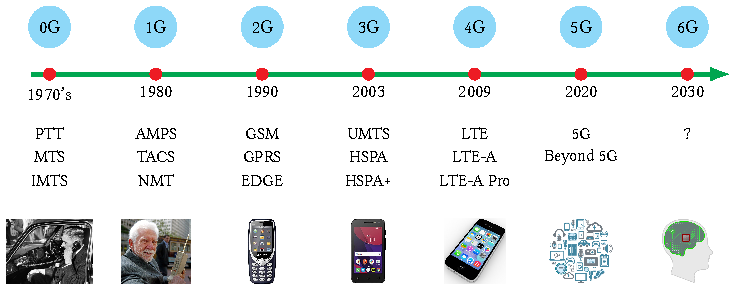
\includegraphics{/Roadmap/mainFig}
\caption{\lofimage{/Roadmap/mainFig}%
حوزه‌های بهینه‌سازی شبکه‌های تلفن همراه از دیدگاه جمع‌آوری داده}
\label{fig:relatedWorksRoadmap}
\end{figure}

\ptext


\section{دیدگاه‌های دسته بندی کارهای پیشین}
\begin{figure}
\begin{subfigure}{.24\textwidth}\centering

\includegraphics{/Person/LukmanMedriavinSilalahi}
\caption{\lr{L. Medriavin Silalahi \cite{silalahi2021improvement}}}
\end{subfigure} 
\begin{subfigure}{.24\linewidth}\centering

\includegraphics{/Person/MarcoSousa}
\caption{\lr{Marco Sousa \cite{Sousa2021Analysis}}}
\end{subfigure}
\begin{subfigure}{.24\linewidth}\centering

\includegraphics{/Person/peeraponguthansakul}
\caption{\lr{Peerapong Uthansakul \cite{charoenlap2016prediction}}}
\end{subfigure}
\begin{subfigure}{.24\linewidth}\centering
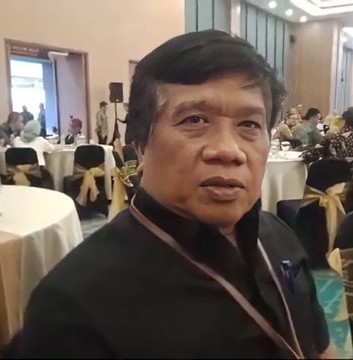
\includegraphics{/Person/YuliarmanSaragih}
\caption{\lr{Yuliarman Saragih \cite{Aprillia2020RF}}}
\end{subfigure}
\end{figure}

\section{ملاک های ارزیابی و مقایسه}

\section{مرور مطالعات موجود}

\section{جمع بندی}

 البته شامل یک جدول مقایسه ای هم باشد با توجه به دیدگاه های دسته بندی و ملاک ها
\end{comment}